%\documentclass{article}
%%\usepackage[english]{babel}%
%\usepackage{graphicx}
%\usepackage{tabulary}
%\usepackage{tabularx}
%\usepackage[table,xcdraw]{xcolor}
%\usepackage{pdflscape}
%\usepackage{lastpage}
%\usepackage{multirow}
%\usepackage{afterpage}
%\usepackage{rotating}
%\usepackage{pdfpages}
%\usepackage{cancel}
%\usepackage{amsmath}
%\usepackage[table]{xcolor}
%\usepackage{caption}
%\captionsetup{font=scriptsize,labelfont=scriptsize}
%\usepackage{pdflscape}
%\usepackage{fixltx2e}
%\usepackage[T1]{fontenc}
%\usepackage[utf8]{inputenc}
%\usepackage{multirow}
%\usepackage{ifthen}
%\usepackage{fancyhdr}
%\usepackage[document]{ragged2e}
%\usepackage[margin=1in,top=1.2in,headheight=57pt,headsep=0.1in]
%{geometry}
%\usepackage{ifthen}
%\usepackage{fancyhdr}
%\everymath{\displaystyle}
%\usepackage[document]{ragged2e}
%\usepackage{fancyhdr}
%\usepackage[table,xcdraw]{xcolor}
%% If you use beamer only pass "xcolor=table" option, i.e. \documentclass[xcolor=table]{beamer}
%\usepackage[normalem]{ulem}
%\useunder{\uline}{\ul}{}
%\everymath{\displaystyle}
%\linespread{2}%controls the spacing between lines. Bigger fractions means crowded lines%
%%\pagestyle{fancy}
%%\usepackage[margin=1 in, top=1in, includefoot]{geometry}
%%\everymath{\displaystyle}
%\linespread{1.3}%controls the spacing between lines. Bigger fractions means crowded lines%
%%\pagestyle{fancy}
%\pagestyle{fancy}
%\setlength{\headheight}{56.2pt}
%
%
%\chead{\ifthenelse{\value{page}=1}{
\includegraphics[scale=0.3]{BassettCTCLogo}\\ \textbf \textbf Water - General Introduction}}
%\rhead{\ifthenelse{\value{page}=1}{Shabbir Basrai}{Shabbir Basrai}}
%\lhead{\ifthenelse{\value{page}=1}{}{\textbf Water - General Introduction}}
%
%
%\cfoot{}
%\lfoot{Page \thepage\ of \pageref{LastPage}}
%\rfoot{}
%\renewcommand{\headrulewidth}{2pt}
%\renewcommand{\footrulewidth}{1pt}
%\newcommand{\comment}[1]{\hspace{0em}{\small\textit{#1}}\bigskip\par}
%\begin{document}


\chapterimage{MathCover.png}
\chapter{Water Math}

\section{Fractions}\index{Fractions}
\begin{itemize}
\item A fraction is defined as part of whole.  If in a class there are 20 male students and 30 male students, the fraction of male students is $\dfrac{20}{50} or \dfrac{2}{5}$.
\item It is composed of three items: two numbers and a line.
\item The number on the top is called the numerator, the number on the bottom is called the denominator, and the line in between them means to divide. 
$$
\text { Divide } \longrightarrow \dfrac{3}{4} \quad \begin{aligned}
&\text { Numerator } \\
&\text { Denominator }
\end{aligned}
$$
\item A proper fraction is a fraction that has no whole number part and its numerator is smaller than its denominator. An improper fraction is a fraction that has a larger numerator than denominator and it represents a number greater than one.\\
Proper Fraction Examples: $\dfrac{1}{2}$, $\dfrac{5}{8}$, $\dfrac{11}{12}$\\
\vspace{0.2cm}
Improper Fraction Examples: $\dfrac{12}{2}$, $\dfrac{5}{2}$
\item Any whole number can be expressed as a fraction by placing a "1" in the denominator. For example:

2 is the same as $\dfrac{2}{1}$ and 45 is the same as $\dfrac{45}{1}$

\item Only fractions with the same denominator can be added/subtracted, and only the numerators are added/subtracted. For example:
$$
\dfrac{1}{8}+\dfrac{3}{8}=\dfrac{4}{8}  \enspace  \text {and},  \enspace \dfrac{7}{8}-\dfrac{3}{8}=\dfrac{4}{8}
$$

\item A fraction combined with a whole number is called a mixed number. For example:
$$
4 \dfrac{1}{8}, \enspace 16 \dfrac{2}{3}, \enspace  8 \dfrac{3}{4}, \enspace  45  \dfrac{1}{2} \text { and, } 12\dfrac{17}{32}
$$
These numbers are read, four and one eighth, sixteen and two thirds, eight and three fourths, forty-five and one half, and twelve and seventeen thirty seconds.\\
Mized numbers 

\item A fraction can be changed by multiplying the numerator and denominator by the same number. This does not change the value of the fraction, only how it looks. For instance:
$$
\dfrac{1}{2} \text { is the same as } \dfrac{1}{2} \times \dfrac{2}{2} \text { which is } \dfrac{2}{4}
$$

\item Steps to convert $\dfrac{17}{4}$ to a mixed number:
\begin{enumerate}[Step 1.]
\item How many times can 4 fit into 17? 4 because 4×4=16.  Thus, 4 becomes the whole number part
\item How much is left over in the numerator? 1 because $17-16=1$.  Thus, 1 becomes the numerator of the fractional part
\item $\dfrac{17}{4} = 4\dfrac{1}{4}$
\end{enumerate}
\vspace{0.2cm}
\item To turn a mixed number into an improper fraction, multiply the whole number part by the denominator and add the numerator. This becomes the new numerator over the original denominator.

Example: Converting 1.5 feet to fraction\\
$1.5ft=1\dfrac{1}{2}$\\
\vspace{0.2cm}
$1\dfrac{1}{2}=\dfrac{1*2+1}{2}=\dfrac{2+1}{2}=\dfrac{3}{2}$
\vspace{0.2cm}
\item A mixed value - say a circumference is given in feet and fraction of feet (say $7 \enspace 3/4$), needs to be converted to a fraction for calculation purposes.
\end{itemize}

\section{Ratio}\index{Ratio}
\begin{itemize}
\item Ratio is used for comparing the size of two or more quantities.
\item Say if there are 10 red cubes and 5 pink marbles in a bag, the ratio $\dfrac{5}{10}$ is the ratio of pink marbles and red cubes.  It can also be represented by 5:10.
\item 5 lbs of chemical in 10 gallons solution is a ratio.  So is 30 miles per gallon.
\item Unlike fractions, ratio does not compare things that have the same units.
\end{itemize}
\section{Proportion}\index{Proportion}
\begin{itemize}
\item Two quantities are said to be in proportion if one changes, the other changes in a specific way.
\item Two quantities are said to be directly proportional, if the \textbf{increase} in one will \textbf{increase} the other value proportionally.  
\begin{itemize}
\item Thus, if two quantities x and y are directly proportional, its ratio $\dfrac{x}{y}$ will be a fixed value. Thus for x$_1$ and y$_1$ different values of x and y respectively will be related by the equation $\dfrac{x}{y}=\dfrac{x_1}{y_1}$.  

\item This relationship is useful for calculating unknown values in water treatment calculations as in the following example: \\
\vspace{0.2cm}
Knowing 200 lbs of bleach is needed to disinfect 5 MG of water at a treatment plant, calculate the lbs of bleach required to disinfect 3.2 MGD flow.\\

\vspace{0.2cm}

The ratio $\dfrac{200 \enspace pounds \enspace bleach}{5 MG}$ or 40 lbs bleach per MG is a constant.  
Using this known proportion the lbs of bleach is needed to disinfect 3.2 MG at this plant can be calculated as follows by setting up the equation as:\\
\vspace{0.2cm}
$\dfrac{40 \enspace pounds \enspace bleach}{MG}=\dfrac{X}{3.2 \enspace MG}$ where X is the unknown lbs of bleach that is required to disinfect the 3.2 MG flow.\\
\vspace{0.2cm}
X can be calculated by cross multiplying the above equation: $X=\dfrac{3.2*40}{1}=128 \enspace lbs \enspace bleach$
\end{itemize}
\item Two quantities are said to be inversely proportional if the \textbf{increase} in one will \textbf{decrease} the other value proportionally.  
\begin{itemize}
\item Thus, if two quantities x and y are inversely proportional, its product $x * \text{y}$ will be a fixed value and different values of x and y respectively will be related by the equation $x *y = x_1 * y_1$.
\item Examples of inversely proportional relationship include:\\
\vspace{0.2cm}
\begin{itemize}
\item Labor hours required to perform a certain task or time required to pump down a wetwell depending on the size of the pump.  An increase in assignment of labor hours will reduce the time required to perform the task 
\item Using a larger pump will reduce the time to pump down the wetwell.  
\item In the Pounds formula:\\
\vspace{0.2cm}
$$lbs \enspace \textbf{or} \enspace \dfrac{lbs}{day}=Concentration\Big(\frac{mg}{l}\Big)*8.34*volume(MG) \enspace \textbf{or} \enspace Flow (MGD)$$\\
 
\vspace{0.2cm}

for the same lbs or lbs/day, concentration varies inversely with volume or flow.  Thus, for a certain pounds added, the concentration will go down if the flow increases and vice versa.
\item In the flow equation, Q=V*A, for the same flow (Q), velocity (V) and surface area (A) are inversely related.  If Q is remaining the same, an increase in surface area will reduce the velocity and vice versa.\\

Additionally, for a flow through a pipe as the surface area of the pipe is proportional to the square of the diameter, the velocity in the pipe is inversely proportional to the square of the diameter.\\

\vspace{0.2cm}

For a constant Q:  $V *A = V_1 *A_1$ or $V *D^2 = V_1 *D_1^2$

\end{itemize}
\vspace{0.2cm}


\vspace{0.2cm}

\item Application of inversely proportional relationship in water related calculation can be demonstration with the following example:

If it takes 20 minutes to pump a wet well down with one pump pumping at 125 gpm, then how long will it take if a 200 gpm pump is used?

As this is an inversely proportional relationship ( a larger pump will reduce the time required):\\
\vspace{0.2cm}
$(20 \mathrm{minutes} * 125 \mathrm{gpm})=(X \mathrm{minutes} * 200 \mathrm{gpm})$ \\

where X is the unknown time to pump down the wetwell with the 200 gpm pump.\\
\vspace{0.2cm}
Solving for X: $X=\dfrac{20*125}{200}=12.5 \enspace \mathrm{minutes}$
\end{itemize}
\end{itemize}
\section{Decimals \& Powers of Ten}\index{Decimals \& Powers of Ten}
\begin{itemize}
\item A decimal is composed of two sets of numbers: the numbers to the left of the decimal are whole numbers, and numbers to the right of the decimal are parts of whole numbers, a fraction of a number.\\

\item The term used to express the fraction component is dependent on the number of characters to the right of the decimal.

\begin{itemize}
  \item The first character after the decimal point is tenths: $0.1$ - tenths

  \item The second character is hundredths: $0.01$ - hundredths

  \item The third character is thousandths: $0.001$ - thousandths
\end{itemize}

\item Powers of 10 notation enables us to work with these very large and small quantities efficiently.
\item In water math, the most common application of this concept is related to parts per million (ppm) or parts per billion (ppb).
\item 1 million - 1,000,000 can be represented as 10$^6$.  Likewise, 1 billion - 1,000, 000,000 can be represented as 10$^9$
\item The sequence of powers of ten can also be extended to negative powers.
\item 1 part per million (1/1,000,000) can be written as 10$^-6$
\end{itemize}



\begin{table}[ht]
\begin{tabular}{|l|l|l|l|l|}
\hline
\multicolumn{1}{|c|}{\textbf{Name}} & \multicolumn{1}{c|}{\textbf{Power}} & \multicolumn{1}{c|}{\textbf{Number}} & \multicolumn{1}{c|}{\textbf{SI symbol}} & \multicolumn{1}{c|}{\textbf{SI prefix}} \\ \hline
one                                 & $10^0$& 1                                    &                                         &                                         \\ \hline
ten                                 & $10^1$                                   & 10                                   & da (D)                                  & deca                                    \\ \hline
hundred                             & $10^2$                                   & 100                                  & h (H)                                   & hecto                                   \\ \hline
thousand                            & $10^3$                                  & 1,000                                & k (K)                                   & kilo                                    \\ \hline
million                             & $10^6$                                   & 1,000,000                            & M                                       & mega                                    \\ \hline
billion                             & $10^9$                                  & 1,000,000,000                        & G                                       & giga                                    \\ \hline
tenth                               & $10^{-1}$                                 & 0.1                                  & d                                       & deci                                    \\ \hline
hundredth                           & $10^{-2}$                                  & 0.01                                 & c                                       & centi                                   \\ \hline
thousandth                          & $10^{-3} $                                 & 0.001                                & m                                       & milli                                   \\ \hline
millionth                           &$10^{-6} $                               & 0.000 001                            & $\mu$                                      & micro                                   \\ \hline
billionth                           & $10^{-9} $                               & 0.000 000 001                        & n                                       & nano                                    \\ \hline
\end{tabular}
\end{table}

\section{Rounding and Significant Digits}\index{Rounding and Significant Digits}

\begin{itemize}
\item Significant digits (also called Significant Figures) are digits which give us useful information about the accuracy of a measurement and are related to rounding.
\item This concept is used to determine the direction to round a number (answer). The basic idea is that no answer can be more accurate than the least accurate piece of data used to calculate the answer.\\
\item Significant digits is the count of the numerals in a measured quantity (counting from the left) whose values are considered as known exactly, plus one more whose value could be one more or one less.\\
\item Rules for determining the number of significant digits:
\begin{enumerate}
\item All nonzero digits are significant:\\
1.234 g has 4 significant figures, and 1.2 g has 2 significant figures.
\item Zeroes between nonzero digits are significant:
1002 kg has 4 significant figures, 3.07 mL has 3 significant figures.
\item Zeroes to the left of the first nonzero digits are not significant; such zeroes merely indicate the position of the decimal point:
\SI{0.001}{\celsius} has only 1 significant figure, 0.012 g has 2 significant figures.
\item Zeroes to the right of a decimal point in a number are significant:
0.023 mL has 2 significant figures, 0.200 g has 3 significant figures.
\item When a number ends in zeroes that are not to the right of a decimal point, the zeroes are not necessarily significant:
190 miles may be 2 or 3 significant figures, 50,600 calories may be 3, 4, or 5 significant figures. The potential ambiguity in the last rule can be avoided by the use of standard exponential, or ”scientific,” notation. For example, depending on whether 3, 4, or 5 significant figures is correct, we could write 50,600 calories as: $5.06*10^4$ calories (3 significant figures) $5.060*10^4$ calories (4 significant figures), or
$5.0600*10^4)$ calories (5 significant figures).
\end{enumerate}
\item Examples of significant figures:
% Please add the following required packages to your document preamble:
% \usepackage[normalem]{ulem}
% \useunder{\uline}{\ul}{}
% Please add the following required packages to your document preamble:
% \usepackage[normalem]{ulem}
% \useunder{\uline}{\ul}{}
\begin{table}[h]
\begin{tabular}{|p{16cm}|}
\hline
\scriptsize{1000 has   one significant digit: only the 1 is interesting (only it tells us anything   specific); we don't know anything for sure about the hundreds, tens, or units   places; the zeroes may just be placeholders; they may have rounded something   off to get this value.                                    } \\ \hline
\scriptsize{1000.0 has five significant   digits: the ".0" tells us something interesting about the presumed   accuracy of the measurement being made; namely, that the measurement is   accurate to the tenths place, but that there happen to be zero tenths.                                                               } \\ \hline
\scriptsize{0.00035 has two significant   digits: only the 3 and 5 tell us something; the other zeroes are   placeholders, only providing information about relative size.                                                                                                                                                    } \\ \hline
\scriptsize{0.000350 has three significant   digits: the last zero tells us that the measurement was made accurate to that   last digit, which just happened to have a value of zero.                                                                                                                                         } \\ \hline
\scriptsize{1006 has four significant   digits: the 1 and 6 are interesting, and we have to count the zeroes, because   they're between the two interesting numbers.                                                                                                                                                          } \\ \hline
\scriptsize{560 has two significant   digits: the last zero is just a placeholder.                                                                                                                                                                                                                                            } \\ \hline
\scriptsize{560. : notice that   "point" after the zero! This has three significant digits, because   the decimal point tells us that the measurement was made to the nearest unit,   so the zero is not just a placeholder.                                                                                                  } \\ \hline
\scriptsize{560.0 has four significant   digits: the zero in the tenths place means that the measurement was made   accurate to the tenths place, and that there just happen to be zero tenths;   the 5 and 6 give useful information, and the other zero is between   significant digits, and must therefore also be counted.} \\ \hline
\end{tabular}
\end{table}
\item Addition and Subtraction\\
\begin{itemize}
\item When you are \hl{adding or subtracting} a bunch of numbers and need to be concerned with significant figures, first add (or subtract) the numbers given in their entire format, and then round the final answer. \hl{When rounding the final answer after adding or subtracting, the answer must be written with the same significant figures as the least accurate decimal place given}.\\
\textbf{Example:} 13.214 + 234.6 + 7.0350 + 6.38\\
\begin{itemize}
\item 13.214 + 234.6 + 7.0350 + 6.38 = 261.2290\\
\item 234.6 is only accurate to the tenths place making it the least accurate number. My answer must be rounded to the same place as the least accurate number:\\
\item 261.2290 rounds to 261.2 (one decimal place)\\
\end{itemize}
\end{itemize}
\item Multiplication and Division\\
\begin{itemize}
\item When \hl{multiplying or dividing} multiple numbers you would do these calculations as normal. When the answer must be written in the appropriate significant figure your answer must \hl{round to the same number of significant figures as the least number of significant figures.}\\
\textbf{Example 1:}  Simplify, and round, to the appropriate number of significant digits \\
\begin{center}
16.235 x 0.217 x 5\\
\end{center}
\begin{enumerate}[Step 1.]
\item First off, 5 has only one significant figure, thus the final answer needs to be rounded to one significant digit\\
\item 16.235 x 0.217 x 5 = 17.614975\\
\item To round 17.614975 to one digit. I'll start with the 1 in the tens place. Immediately to its right is a 7, which is greater than 5, so 1 is rounded up to 2, and then replacing the 7 with a zero, and dropping the decimal point and everything after it.
\item 17.614975 rounds to 20\\
\end{enumerate}
\textbf{Example 2:}  Simplify, and round, to the appropriate number of significant figures\\
\begin{center}
0.00435 x 4.6
\end{center}
\begin{enumerate}[Step 1.]
\item 4.6 has only 2 significant figures, so the final answer should be rounded to two significant figures.
\item 0.00435 x 4.6 = 0.02001\\
\item 0.02001 would round to 0.020, which has 2 significant figures (0.020). The answer cannot be 0.02, because that value would have only one significant figure.\\
\end{enumerate}
\end{itemize}
\end{itemize}

\begin{itemize}
\item \emph{A number is rounded off by dropping one or more numbers from the right and adding zeroes, if necessary, to maintain the decimal point.} 
\item \emph{If the last figure dropped is 5 or more, increase the last retained figure by 1. If the last digit dropped is less than 5, do not increase the last retained figure.}
\end{itemize}


\section{Averages}\index{Averages}
\begin{itemize}
\item Also known as \emph{arithmetic mean}, this value is arrived at by adding the quantities in a series and dividing the total by the number in the series.
\end{itemize}
Example 1: Find the average of the following series of numbers: 12,8,6,21,4,5 , 9 , and 12.\\
Adding the numbers together we get 77.\\
There are 8 numbers in this set.\\
Divide 77 by 8.\\

$\frac{77}{8}=9.6$ is the average of the set\\

Example 2:  Find the average of the set of daily turbidity data - 0.3,0.4,0.3,0.1,and 0.8\\
The total is 1.9.\\
There are 5 numbers in the set.\\
Therefore:
$$
\frac{1.9}{5}=0.38, \text { rounding off }=0.4
$$

\section{Working with Percent}\index{Working with Percent}
\begin{itemize}
\item Percent expresses portions of the whole.  
\item \texthl{The whole is considered as 1 or 100\% and a part of the whole can be expressed as a percent.}
\textbf{Example:} If a tank is $1 / 2$ full, we say that it contains $50 \%$ of the original solution.
\item Percentage is written as a whole number with a \% sign after it. 
\item In a calculation, percent is expressed as a decimal. 
\item \texthl{The decimal form of a percent value is obtained by dividing the percent by 100.}\\
 \textbf{Example:} $11 \%$ is expressed as the decimal $0.11$, since $11 \%$ is equal to $11 / 100$. This decimal is obtained by dividing 11 by 100.
\item \texthl{To determine what percentage a part is of the whole, divide the part by the whole.}\\
\textbf{Example:} There are 80 water meters to read, Jim has finished 24 of them. What percentage of the meters have been read?\\
$$24 \div 80=0.30$$\\
The $0.30$ is converted to percent by multiplying the answer by 100.\\
$$0.30 \times 100=30 \%$$\\
Thus $30 \%$ of the 80 meters have been read.\\

\item \texthl{To find the percentage of a number, multiply the number by the decimal equivalent of the percentage given in the problem.}\\
\textbf{Example:}\\
What is $28 \%$ of $286 ?$\\

\begin{enumerate}[Step 1.]
\item Change the $28 \%$ to a decimal equivalent:  $$28 \% \div 100=0.28$$
\item Multiply $286 \times 0.28=80$\\
Thus $28 \%$ of 286 is 80.
\end{enumerate}

\item \texthl{To increase a value by a percent, add the decimal equivalent of the percent to " 1 " and multiply it times the number.}

\textbf{Example:} A filter bed will expand $25 \%$ during backwash. If the filter bed is 36 inches deep, how deep will it be during backwash?\\

\begin{enumerate}[Step 1.]
\item Change the percent to a decimal.
$$
25 \% \div 100=0.25
$$
\item Add the whole number 1 to this value.
$$
1+0.25=1.25
$$
\item Multiply times the value.
$$
36 \text { in } \times 1.25=45 \text { inches }
$$
\end{enumerate}
\end{itemize}
\subsection{Percentage Concentrations}
Above concepts are used for chemicals such as fluoride and hypochlorites - the strength of the product as used is commonly expressed as a percentage.

\textbf{Example 1:} A chlorine solution was made to have a $4 \%$ concentration. It is often desirable to determine this concentration in $\mathrm{mg} / \mathrm{L}$. This is relatively simple: the $4 \%$ is four percent of a million.

To find the concentration in $\mathrm{mg} / \mathrm{L}$ when it is expressed in percent, do the following:

\begin{enumerate}
  \item Change the percent to a decimal.
\end{enumerate}
$$
4 \% \div 100=0.04
$$

\begin{enumerate}
  \setcounter{enumi}{2}
  \item Multiply times a million.
\end{enumerate}
$$
0.04 \times 1,000,000=40,000 \mathrm{mg} / \mathrm{L}
$$
We get the million because a liter of water weighs $1,000,000 \mathrm{mg} .1 \mathrm{mg}$ in 1 liter is 1 part in a million parts ( $\mathrm{ppm}) .1 \%=10,000 \mathrm{mg} / \mathrm{L}$.


\textbf{Example 2:} How much $65 \%$ calcium hypochlorite is required to obtain 7 pounds of pure chlorine?\\
$65 \%$ implies that in every lb of calcium hypochlorite has $65 \%$ lbs of available chlorine.\\
\vspace{0.2cm}
Therefore, $\dfrac{0.65 \textrm{ lbs available chlorine}}{\textrm{lb of calcium hypochlorite}} $ or conversely $\dfrac{\textrm{lb of calcium hypochlorite}}{0.65 \textrm{ lbs available chlorine}}$\\
\vspace{0.2cm}
$\implies{\textrm{lbs calcium hypchlorite required}}=\dfrac{\textrm{lb of calcium hypochlorite}}{0.65 \cancel{\textrm{ lbs available chlorine}}}*\dfrac{7\cancel{\textrm{ lb of available chlorine}}}{}$\\
\vspace{0.2cm}
$=\boxed{10.8 \textrm{ lbs of calcium hypochlorite with } 65\%\textrm{available chlorine is required}}$

\section{Area \& Volume}\index{Area \& Volume}
% \section{Area \& Volume}\index{Area \& Volume}

% \begin{snugshade*}
% 	\item \noindent\textsc{Area \& Volume}
% \end{snugshade*}

\begin{center}
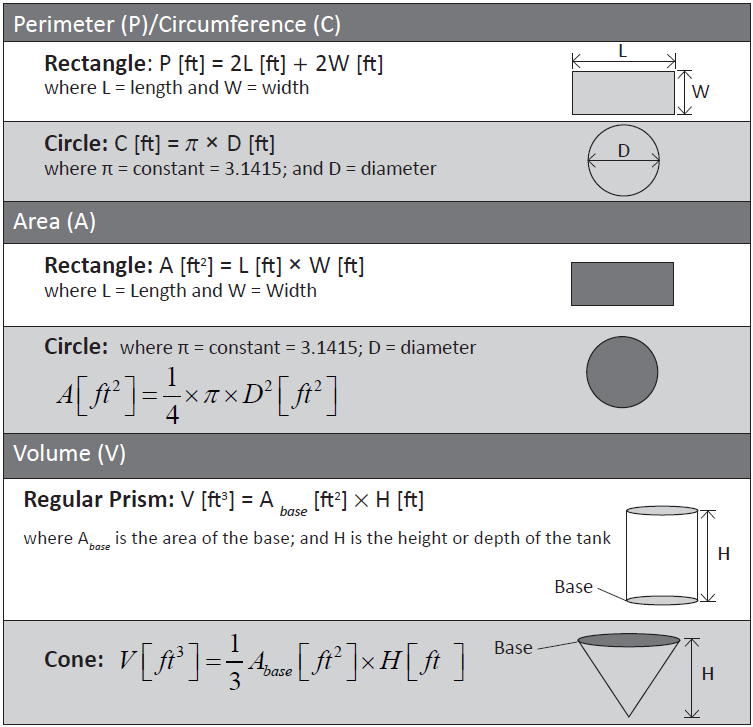
\includegraphics[scale=0.5]{Area&VolumeFormula}
\end{center}
\textbf{Example 1:} The floor of a rectangular building is 20 feet long by 12 feet wide and the inside walls are 10 feet high. Find the total surface area of the inside walls of this building\\
Solution:\\
% \begin{center}
\begin{tikzpicture}
	%%% Edit the following coordinate to change the shape of your
	%%% cuboid
      
	%% Vanishing points for perspective handling
	\coordinate (P1) at (-7cm,1.5cm); % left vanishing point (To pick)
	\coordinate (P2) at (8cm,1.5cm); % right vanishing point (To pick)

	%% (A1) and (A2) defines the 2 central points of the cuboid
	\coordinate (A1) at (0em,0cm); % central top point (To pick)
	\coordinate (A2) at (0em,-2cm); % central bottom point (To pick)

	%% (A3) to (A8) are computed given a unique parameter (or 2) .8
	% You can vary .8 from 0 to 1 to change perspective on left side
	\coordinate (A3) at ($(P1)!.8!(A2)$); % To pick for perspective 
	\coordinate (A4) at ($(P1)!.8!(A1)$);

	% You can vary .8 from 0 to 1 to change perspective on right side
	\coordinate (A7) at ($(P2)!.7!(A2)$);
	\coordinate (A8) at ($(P2)!.7!(A1)$);

	%% Automatically compute the last 2 points with intersections
	\coordinate (A5) at
	  (intersection cs: first line={(A8) -- (P1)},
			    second line={(A4) -- (P2)});
	\coordinate (A6) at
	  (intersection cs: first line={(A7) -- (P1)}, 
			    second line={(A3) -- (P2)});

	%%% Depending of what you want to display, you can comment/edit
	%%% the following lines

	%% Possibly draw back faces

	\fill[gray!40] (A2) -- (A3) -- (A6) -- (A7) -- cycle; % face 6
	\node at (barycentric cs:A2=1,A3=1,A6=1,A7=1) {\tiny Floor=W*L};
	
	\fill[gray!50] (A3) -- (A4) -- (A5) -- (A6) -- cycle; % face 3
	\node at (barycentric cs:A3=1,A4=1,A5=1,A6=1) {\tiny Wall - W*H};
	
	\fill[gray!10, opacity=0.2] (A5) -- (A6) -- (A7) -- (A8) -- cycle; % face 4
	\node at (barycentric cs:A5=1,A6=1,A7=1,A8=1) {\tiny Wall - L*H};
	
	\fill[gray!10,opacity=0.5] (A1) -- (A2) -- (A3) -- (A4) -- cycle; % f2
	\node at (barycentric cs:A1=1,A2=1,A3=1,A4=1) {\tiny Wall - L*H};
	
	\fill[gray!40,opacity=0.2] (A1) -- (A4) -- (A5) -- (A8) -- cycle; % f5
	\node at (barycentric cs:A1=1,A4=1,A5=1,A8=1) {\tiny Ceiling=W*L};	
	
	\draw[thick,dashed] (A5) -- (A6);
	\draw[thick,dashed] (A3) -- (A6);
	\draw[thick,dashed] (A7) -- (A6);

	%% Possibly draw front faces

	%\fill[orange] (A1) -- (A8) -- (A7) -- (A2) -- cycle; % face 1
	\node at (barycentric cs:A1=1,A8=1,A7=1,A2=1) {\tiny Wall - W*H};
	


	%% Possibly draw front lines
	\draw[thick] (A1) -- (A2);

	\draw[<->] (-1.8,0.38) -- (-1.8,-1.3)node [midway, above=-1.8mm] {\hspace{-1.3cm}\tiny Height=10'};
	\draw[<->] (-1.6,-1.4) -- (-.3,-2.1)node [midway, above=-2.6mm] {\hspace{-1.3cm}\tiny Length=20'};
	\draw[<->] (2.6,-1.13) -- (0.2,-2.2)node [midway, below=.6mm] {\hspace{1.2cm}\tiny Width=12'};
	\draw[thick] (A3) -- (A4);
	\draw[thick] (A7) -- (A8);
	\draw[thick] (A1) -- (A4);
	\draw[thick] (A1) -- (A8);
	\draw[thick] (A2) -- (A3);
	\draw[thick] (A2) -- (A7);
	\draw[thick] (A4) -- (A5);
	\draw[thick] (A8) -- (A5);
	
	% Possibly draw points
	% (it can help you understand the cuboid structure)
%	\foreach \i in {1,2,...,8}
%	{
%	  \draw[fill=black] (A\i) circle (0.15em)
%	    node[above right] {\tiny \i};
%	}
	% \draw[fill=black] (P1) circle (0.1em) node[below] {\tiny p1};
	% \draw[fill=black] (P2) circle (0.1em) node[below] {\tiny p2};
\end{tikzpicture}\\
% \end{center}
2 Walls W*H + 2 Walls L*H= $2*12*10ft^2 + 2*20*10ft^2$\\
$=240+400=\boxed{640ft^2}$\\

2 Walls W*H + 2 Walls L*H + Floor + Ceiling= $2*12*10ft^2 + 2*20*10ft^2 + 2*12*20ft^2$\\
$=240+400+480=\boxed{1,120ft^2}$\\

\textbf{Example 2:} How many gallons of paint will be required to paint the inside walls of a 40 ft long x 65 ft wide x 20 ft high tank if the paint coverage is 150 sq. ft per gallon.  Note:  We are painting walls only.  Disregard the floor and roof areas.\\
Solution:\\
\vspace{0.3cm}
% \begin{center}
\begin{tikzpicture}
	%%% Edit the following coordinate to change the shape of your
	%%% cuboid
      
	%% Vanishing points for perspective handling
	\coordinate (P1) at (-7cm,1.5cm); % left vanishing point (To pick)
	\coordinate (P2) at (8cm,1.5cm); % right vanishing point (To pick)

	%% (A1) and (A2) defines the 2 central points of the cuboid
	\coordinate (A1) at (0em,0cm); % central top point (To pick)
	\coordinate (A2) at (0em,-2cm); % central bottom point (To pick)

	%% (A3) to (A8) are computed given a unique parameter (or 2) .8
	% You can vary .8 from 0 to 1 to change perspective on left side
	\coordinate (A3) at ($(P1)!.8!(A2)$); % To pick for perspective 
	\coordinate (A4) at ($(P1)!.8!(A1)$);

	% You can vary .8 from 0 to 1 to change perspective on right side
	\coordinate (A7) at ($(P2)!.7!(A2)$);
	\coordinate (A8) at ($(P2)!.7!(A1)$);

	%% Automatically compute the last 2 points with intersections
	\coordinate (A5) at
	  (intersection cs: first line={(A8) -- (P1)},
			    second line={(A4) -- (P2)});
	\coordinate (A6) at
	  (intersection cs: first line={(A7) -- (P1)}, 
			    second line={(A3) -- (P2)});

	%%% Depending of what you want to display, you can comment/edit
	%%% the following lines

	%% Possibly draw back faces

	\fill[gray!40] (A2) -- (A3) -- (A6) -- (A7) -- cycle; % face 6
	\node at (barycentric cs:A2=1,A3=1,A6=1,A7=1) {};
	
	\fill[gray!50] (A3) -- (A4) -- (A5) -- (A6) -- cycle; % face 3
	\node at (barycentric cs:A3=1,A4=1,A5=1,A6=1) {\tiny Wall - W*H};
	
	\fill[gray!10, opacity=0.2] (A5) -- (A6) -- (A7) -- (A8) -- cycle; % face 4
	\node at (barycentric cs:A5=1,A6=1,A7=1,A8=1) {\tiny Wall - L*H};
	
	\fill[gray!10,opacity=0.5] (A1) -- (A2) -- (A3) -- (A4) -- cycle; % f2
	\node at (barycentric cs:A1=1,A2=1,A3=1,A4=1) {\tiny Wall - L*H};
	
	\fill[gray!40,opacity=0.2] (A1) -- (A4) -- (A5) -- (A8) -- cycle; % f5
	\node at (barycentric cs:A1=1,A4=1,A5=1,A8=1) {};	
	
	\draw[thick,dashed] (A5) -- (A6);
	\draw[thick,dashed] (A3) -- (A6);
	\draw[thick,dashed] (A7) -- (A6);

	%% Possibly draw front faces

	%\fill[orange] (A1) -- (A8) -- (A7) -- (A2) -- cycle; % face 1
	\node at (barycentric cs:A1=1,A8=1,A7=1,A2=1) {\tiny Wall - W*H};
	


	%% Possibly draw front lines
	\draw[thick] (A1) -- (A2);

	\draw[<->] (-1.8,0.38) -- (-1.8,-1.3)node [midway, above=-1.8mm] {\hspace{-1.3cm}\tiny Height=20'};
	\draw[<->] (-1.6,-1.4) -- (-.3,-2.1)node [midway, above=-2.6mm] {\hspace{-1.3cm}\tiny Length=40'};
	\draw[<->] (2.6,-1.13) -- (0.2,-2.2)node [midway, below=.6mm] {\hspace{1.2cm}\tiny Width=65'};
	\draw[thick] (A3) -- (A4);
	\draw[thick] (A7) -- (A8);
	\draw[thick] (A1) -- (A4);
	\draw[thick] (A1) -- (A8);
	\draw[thick] (A2) -- (A3);
	\draw[thick] (A2) -- (A7);
	\draw[thick] (A4) -- (A5);
	\draw[thick] (A8) -- (A5);
	
	% Possibly draw points
	% (it can help you understand the cuboid structure)
%	\foreach \i in {1,2,...,8}
%	{
%	  \draw[fill=black] (A\i) circle (0.15em)
%	    node[above right] {\tiny \i};
%	}
	% \draw[fill=black] (P1) circle (0.1em) node[below] {\tiny p1};
	% \draw[fill=black] (P2) circle (0.1em) node[below] {\tiny p2};
\end{tikzpicture}\\
% \end{center}
\vspace{0.3cm}
2 Walls W*H + 2 Walls L*H = $2*65*20ft^2 + 2*40*20ft^2= 2,600+1,600=4,200ft^2$\\
$\implies @150\dfrac{ft^2}{gal} \enspace paint \enspace coverage \enspace \rightarrow \enspace \dfrac{4,200\cancel{ft^2}}{150\dfrac{\cancel{ft^2}}{gal}}=\boxed{28 \enspace gallons}$
\vspace{0.3cm}
\textbf{Example 3:}  What is the circumference of a 100 ft diameter circular sedimentation tank?\\
\vspace{0.3cm}
Solution:\\
\vspace{0.3cm}
$Circumference=\pi*D=3.14*100ft=\boxed{314ft}$
\vspace{0.3cm}

\textbf{Example 4:} If the surface area of a clarifier is 5,025$ft^2$, what is its diameter?\\
\vspace{0.3cm}
Solution:\\
\vspace{0.3cm}
$Surface \enspace area=\dfrac{\pi}{4}*D^2 \enspace \implies 5025(ft^2)=0.785*D^2 (ft^2)$\\
$\implies D^2=\dfrac{5025}{0.785} \implies D=\sqrt{6401.3}=\boxed{80ft}$
\vspace{0.3cm}

\textbf{Example 5:} How many gallons of water would 600 feet of 6-inch diameter pipe hold, approximately?\\
\vspace{0.3cm}
Solution:\\

\vspace{0.3cm}
% \begin{center}
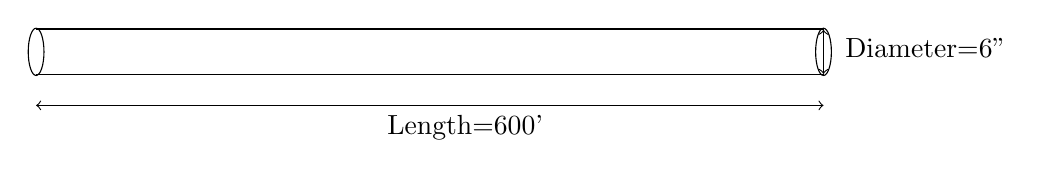
\begin{tikzpicture}
\draw (0,0) ellipse (0.1cm and 0.3cm);
\draw (10,0) ellipse (0.1cm and 0.3cm);
\draw [-] (0,-0.29) -- (10,-0.29);
\draw [-] (0,0.29) -- (10,0.29);
\draw [<->] (10,-0.28) -- (10,0.28) node [midway, below=-3mm] {\hspace{2.6cm}Diameter=6"};
\draw [<->] (0,-.68) -- (10,-.68)node [midway, below] {\hspace{0.9cm}Length=600'};
\end{tikzpicture}
% \end{center}
\vspace{0.3cm}
$Volume=\dfrac{\pi}{4}D^2*L=0.785*\Big(\dfrac{6}{12}\Big)^2*600\cancel{ft^3}*7.48\dfrac{gallons}{\cancel{ft^3}}=\boxed{881 \enspace gallons}$


\section{Flow and Velocity}\index{Flow and Velocity}
\begin{itemize}
\item Flow Rate - Q (volume/time) = velocity (distance or length traveled /time) * surface area
\item Velocity is the speed at which the water is flowing.  It is measured in units of length/time – ft./sec.
\item Velocity of water flowing through can be calculated by dividing the flow rate by area of the flow stream.\\
\vspace{0.5cm}
$$Velocity \enspace \dfrac{length}{time}= \dfrac{flow \enspace rate(\dfrac{volume \enspace or \enspace cubic \enspace length}{time})}{surface \enspace area \enspace in \enspace the \enspace direction \enspace of \enspace flow-square \enspace length}$$
\vspace{0.5cm}
\textbf{For a flow in a channel:}\\
\vspace{0.5cm}
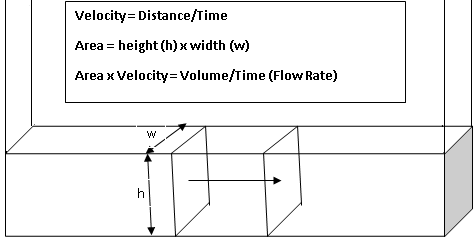
\includegraphics[scale=0.5]{ChannelFlow3}\\

\textbf{For a flow in a pipe:}\\
\vspace{0.5cm}
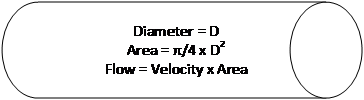
\includegraphics[scale=0.65]{VelocityinPipe}\\
\vspace{0.5cm}
\end{itemize}

\textbf{Example 1:} If a chemical is added in a pipe where water is flowing at a velocity of 3.1 feet per second, how many minutes would it take for the chemical to reach a point 7 miles away?  \\

Note - we want the answer in minutes\\

$$\textrm{Min } = \dfrac{1}{3.1}\dfrac{sec}{ft}*\dfrac{5280ft}{mile}*7 miles*\dfrac{min}{60 sec} = \boxed{199 min}$$
\\

\textbf{Example 2:} Find the flow in cfs in a 6 -inch line, if the velocity is 2 feet per second.

\begin{enumerate}
\item Determine the cross-sectional area of the line in square feet. Start by converting the diameter of the pipe to inches.

The diameter is 6 inches: therefore, the radius is 3 inches. 3 inches is $3 / 12$ of a foot or $0.25$ feet.

\item Now find the area in square feet.
$$
\begin{aligned}
&A=\pi \times r^{2} \\
&A=\pi \times\left(0.25 \mathrm{ft}^{2}\right. \\
&A=\pi \times 0.0625 \mathrm{ft}^{2} \\
&A=0.196 \mathrm{ft}^{2}
\end{aligned}
$$
Or
$$
\begin{aligned}
&A=0.785 \times D^{2} \\
&A=0.785 \times 0.5^{2} \\
&A=0.785 \times .05 \times .05 \\
&A=0.196 \mathrm{ft}^{2}
\end{aligned}
$$

\item Now find the flow.

$\mathrm{Q}=\mathrm{V} \times \mathrm{A}$

$\mathrm{Q}=2 \mathrm{ft} / \mathrm{sec} \times 0.196 \mathrm{ft}^{2}$

$\mathrm{Q}=0.3927 \mathrm{cfs}$ or $0.4 \mathrm{cfs}$
\end{enumerate}


\section{Concentration}\index{Concentration}
\begin{itemize}
\item Concentration is typically expressed as mg/l which is the weight of the constituent (mg) in 1 liter of water.
\item As 1 liter of water weighs 1 million mg, a concentration of 1 mg/l implies 1 mg of constituent per 1 million mg of water or one part per million (ppm).   \texthl{Thus, mg/l and ppm are synonymous.}
\item Sometimes the constituent concentration is expressed in terms of percentage.\\
\vspace{6pt}
\textbf{Example:} 12.5\% chlorine concentration solution.\\
\vspace{0.2cm}
100\% would mean 1,000,000 mg/l or 1,000,000 ppm\\
\vspace{0.2cm}
$\implies$1\% would be $\dfrac{1,000,000}{100}\textrm{mg/l} = \textrm{10,000 mg/l or 10,000 ppm}$\\
\vspace{0.2cm}
$\implies$12.5\% chlorine concentration is 125,000 mg/l or 125,000 ppm.
\vspace{6pt}

$1\% \enspace concentration = 10,000 \enspace ppm \enspace or \enspace\dfrac{mg}{l}$\\
$0.1\% \enspace concentration = 1,000 \enspace ppm \enspace or \enspace \dfrac{mg}{l}$\\
$0.01\% \enspace concentration = 100 \enspace ppm \enspace or \enspace \dfrac{mg}{l}$\\
$10\% \enspace concentration = 100,000 \enspace ppm \enspace or \enspace \dfrac{mg}{l}$\\
$5\% \enspace concentration = 50,000 \enspace ppm \enspace or \enspace \dfrac{mg}{l}$\\
$12.5\% \enspace concentration = 125,000 \enspace ppm \enspace or \enspace \dfrac{mg}{l}$\\
\end{itemize}

\section{Density}\index{Density}
\begin{itemize}
\item Density is defined as the weight of a substance per a unit of its volume. For example, pounds per cubic foot or pounds per gallon.

\item Here are a few key facts about density:
\begin{itemize}

\item Density is measured in units of lb/ft3, lb/gal, or mg/L. Density of water = 62.4 lb/ft3 = 8.34 lb/gal.
\end{itemize}
\end{itemize}

\section{Specific Gravity}\index{Specific Gravity}
\begin{itemize}
\item Specific gravity is the ratio of the density of a substance (liquid or solid) to the density water.
\item It is the ratio of the weight of the substance of a certain volume to the weight of water of the same volume.

\item Any substance with a density greater than that of water will have a specific gravity greater than 1.0. Any substance with a density less than that of water will have a specific gravity less than 1.0. 

\item Specific gravity examples:
\begin{itemize}

\item Specific gravity of water = 1.0 
\item Specific gravity of concrete = 2.5 (depending on ingredients)
\item Specific gravity of alum (liquid @ 60°F) = 1.33 
\item Specific gravity of hydrogen peroxide (35\%) = 1.132
\end{itemize}

\item Specific gravity is used in two ways:
\begin{enumerate}
\item To calculate the total weight of a \% solution (either as a single gallon or a drum volume).\\
Total Weight = Drum Vol X SG X 8.34
\item To calculate the “active ingredient” weight of a single gallon or a drum.\\

Active Ingredient Weight within Drum = Drum Volume X SG X 8.34 X \% solution as a decimal. (i.e., Total Weight X \% solution as a decimal)\\

NOTE: Both ways start with solving for the total weight (Drum Vol X SG X 8.34). When solving for “active ingredient” weight, you have to then multiply by \% solution as a decimal.

\end{enumerate}
\end{itemize}

\textbf{Example:} What is the weight of 5 gallons of a 40\% ferric chloride solution given its specific gravity of 1.43?
$$(8.34 * 1.43) \enspace lbs/gal*5 \enspace gallons = \boxed{59.6 \enspace lbs}$$

The weight of active ferric chloride in the drum will be 59.6*0.4=23.84 lbs (as ferric chloride is 40\% strength)

\section{Detention Time}\index{Detention Time}
\begin{itemize}
\item \colorbox{lime}{Detention Time} - The actual or theoretical (calculated) time required for water to fill a tank at a given flow; pass through a tank at a given flow; or remain in a settling basin, flocculating basin, rapid-mix chamber, or storage tank.\\
$$Tank/clarifier \enspace detention \enspace time \enspace (hr) = 	\dfrac{ Tank/clarifier \enspace volume (cu.ft \enspace or \enspace gal)}{Influent \enspace flow \enspace (cu.ft \enspace or \enspace gal)/hr)}$$
Rectangular tank/clarifier volume = width * length * depth of water\\
Circular tank/clarifier volume = 0.785 * Diameter$^2$ * depth of water\\
Typically volume is calculated in cu. ft and influent flow is given in gallons.  Use 7.48 gal/ft$^3$ conversion factor to convert volume in cu. ft to gallons.\\
\end{itemize}


\section{Unit Conversions}\index{Unit Conversions}
\begin{itemize}
\item A conversion is a number that is used to multiply or divide into a measure in order to change the units of the original measure.

\begin{table}[h!]

\begin{center}
    \begin{tabular}{ | p{4cm} |p{8cm}|}
    \hline
    
\textbf{Measure} & \textbf{Units}\\
\hline   
Length  & inches, ft, miles\\
\hline 
Area  & ft$^2$, acres \\
\hline 
Volume & ft$^3$, gallons, acres-ft.\\
\hline 
Density & weight per volume, lbs/ft$^3$, lbs/gallon\\
\hline 
Flow & ft$^3$/min, MGD, acres-ft/day\\
\hline 

	

    \end{tabular}
 \caption{Common units in water calculations}	
    \end{center}

    \end{table}

\item In most instances, the conversion factor cannot be derived. It must be known. Therefore, tables such as the one below are used to find the common conversions.\\
\begin{tabular}{|l|l|}
\hline
Some Common Conversions & Weight \\
\hline
Linear Measurements & $1 \mathrm{ft}^{3}$ of water $=62.4 \mathrm{lbs}$ \\
\hline
1 inch $=2.54 \mathrm{~cm}$ & $1 \mathrm{gal}=8.34 \mathrm{lbs}$ \\
$1 \mathrm{foot}=30.5 \mathrm{~cm}$ & $1 \mathrm{lb}=453.6 \mathrm{grams}$ \\
$1 \mathrm{~meter}=100 \mathrm{~cm}=3.281 \mathrm{feet}=39.4$ inches 1 & $1 \mathrm{~kg}=1000 \mathrm{~g}=2.2 \mathrm{lbs}$ \\
acre $=43,560 \mathrm{ft}^{2}$ & $1 \%=10,000 \mathrm{mg} / \mathrm{L}$ \\
$1 \mathrm{yard}=3 \mathrm{feet}$ & $1 \mathrm{pound}=16 \mathrm{oz} \mathrm{dry} \mathrm{wt}$ \\
 & $1 \mathrm{ft}^{3}=62.4 \mathrm{lbs}$ \\
\hline
Volume & Pressure \\
\hline
$1 \mathrm{gal}=3.78$ liters & $1 \mathrm{ft}$ of head $=0.433 \mathrm{psi}$ \\
$1 \mathrm{ft}=7.48$ gal & $1 \mathrm{psi}=2.31 \mathrm{ft}$ of head \\
$1 \mathrm{~L}=1000 \mathrm{~mL}$ &  \\
$1 \mathrm{gal}=16 \mathrm{cups}$ &  \\
\hline
Flow &  \\
\hline
$1 \mathrm{cfs}=448 \mathrm{gpm}$ &  \\
$1 \mathrm{gpm}=1440 \mathrm{gpd}$ &  \\
\hline
\end{tabular}
\vspace{0.2cm}
\item Common conversions in water related calculations include the following:

\begin{itemize}
  \item gpm to cfs

  \item Million gallons to acre feet

  \item Cubic feet to acre feet

  \item Cubic feet of water to gallons


  \item gpm to MGD 

  \item psi to feet of head

\end{itemize}

\item Steps for unit conversion:\\
\begin{enumerate}[Step 1:]
\item \texthl{Make sure the original unit is for the same measurement as the converted (desired) unit.}  So if the original unit is for area, say in ft$^2$ the converted unit should be another area unit such as in$^2$ or acre but it cannot be gallons as gallon is a unit of volume.\\
Note:  Calculating the weight of a certain volume of water involves the use of density which is the mass per volume -  value in units including lbs/gallon or lbs/$ft^3$\\

\item Write down the conversion formula as:\\

$Quantity \enspace in \enspace converted \enspace unit = Quantity \enspace (\cancel{Original \enspace Unit}) *   Conversion  \enspace Factor \enspace  \dfrac{Conversion \enspace unit}{\cancel{Original \enspace unit}}$\\
\end{enumerate}

\item Note:  If you wish to convert cubic feet of water to pounds, you have to use its density which is the known mass per unit volume.\\
$\dfrac{8.34 \enspace lbs}{gallon}$ or $\dfrac{62.4 \enspace lbs}{ft^3}$\\
$mass \enspace of \enspace water = \cancel{Volume} *   Density  (\dfrac{mass}{\cancel{Volume}})$\\

\end{itemize}

Example Problems:\\
\begin{enumerate}
\item Convert 1000 $ft^3$ to cu. yards\\

$1000 \cancel{ft^3}*\dfrac{cu.yards}{27\cancel{ft^3}} = 37 cu.yards$

\item Convert 10 gallons/min to $ft^3$/hr\\
Note:  This involves use of two conversion factors - one for converting gallons to cubic feet and another for converting minute to gallons.\\ 
$\dfrac{10 \cancel{gallons}}{\cancel{min}}*  \dfrac{ft^3}{7.48 \cancel{gallons}}  * \dfrac{60 \cancel{min}}{hr}   = \dfrac{80.2ft^3}{hr}$


\item Convert 100,000 $ft^3$ to acre-ft.\\
$100,000 \cancel{ft^3} * \dfrac{acre-ft}{43,560 \cancel{ft^2-ft}} =  2.3 acre-ft$\\

\item Convert 8 $ft^3$ of water to pounds.\\
Here the conversion is from a volume ($ft^3$) to a weight (lbs).  It involves use of a standard correlation of the volume of water to its weight - its density. 

$Weight \enspace of \enspace water \enspace in \enspace lbs=8 \cancel{ft^3} *   62.4  (\dfrac{lbs}{\cancel{ft^3}}) = 499.2 \enspace lbs $\\

\end{enumerate}

\section{Pounds Formula}



Pounds formula is used for:
\begin{itemize}
\item Calculating the quantity in pounds of a particular wastewater constituent entering or leaving a wastewater treatment process
\item Calculating the pounds of chemicals to be added\\
\end{itemize}
So if the concentration of a particular constituent (in mg/liter) and the volume or flow of wastewater is given, one can calculate the amount of that constituent in pounds using the following – Pounds Formula:
$$lbs \enspace \textbf{or} \enspace \dfrac{lbs}{day}=concentration(\dfrac{mg}{l})*8.34*volume(MG) \enspace \textbf{or} \enspace flow(\dfrac{MG}{day}(MGD)$$

\begin{figure}[h!]
\begin{center}
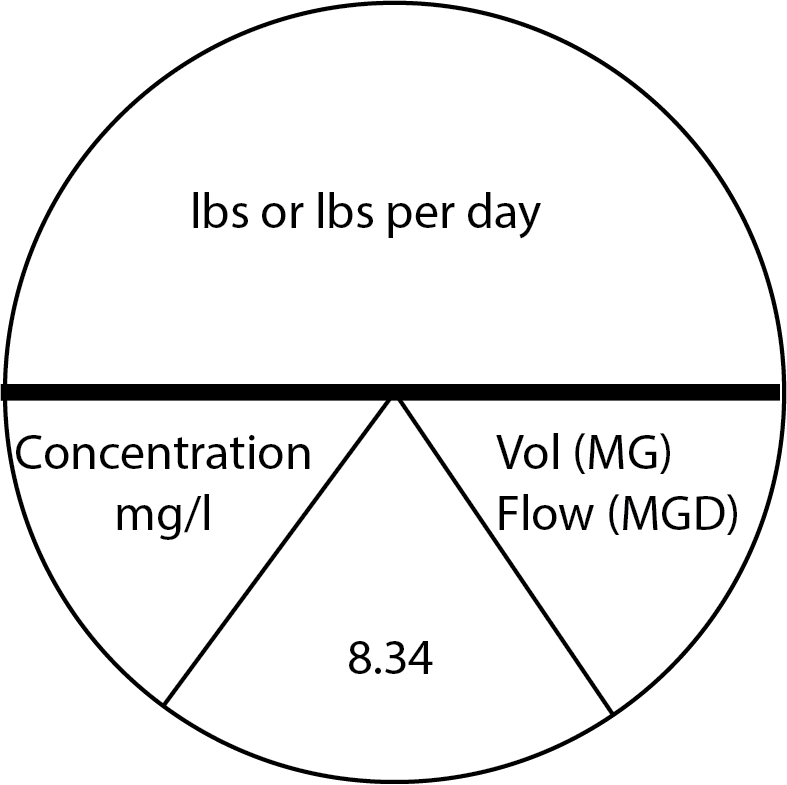
\includegraphics[scale=0.5]{PoundsFormula}
\end{center}
\caption{Pounds formula "nomograph"}
\end{figure}
\vspace{0.3cm}
There are three variables – (lbs, concentration and volume) and one constant (8.34) in the pounds formula.  Knowing any of the two variables in the formula, one can calculate the third (unknown) variable by rearranging the equation.
\subsection{Example Problems}
% \hl{Example Problems}\\
\begin{enumerate}

\item If the influent wastewater flow is 5 MGD and the BOD concentration is 240 mg/l what is the daily BOD loading in lbs/day?\\
Solution:\\
$\dfrac{lbs \enspace BOD}{day}=5MGD*240mg/l*8.34=\boxed{\dfrac{10,000lbs}{day}}$\\

\item Calculate the lbs of solids in the primary sludge if the sludge flow is 7500 gallons and the solids concentration is 4.5\%.\\
Solution\\
Applying lbs formula:\\
$lbs \enspace solids = \dfrac{7500 \enspace MG}{1,000,000} * 4.5*10,000 *8.34 = \boxed{2,815 \enspace lbs \enspace solids}$\\
\textbf{Note:}\\  
1) 7500 gallons was converted to MG by dividing by 1,000,000\\
$7500 \enspace gallons * \dfrac{1 MG}{1,000,000 \enspace gallons}$\\
2) 4.5\% was converted to mg/l by multiplying by 10,000 as 1\%=10,000mg/l

\item An operator dissolves 1,200 lbs of a chemical in 12,000 gallons of water, what is the resultant concentration in mg/l, of the chemical solution?\\
Solution:\\
$Concentration \enspace \dfrac{mg}{l}=\dfrac{lbs}{Volume \enspace MG \enspace * \enspace 8.34}$\\
$Concentration \enspace \dfrac{mg}{l}=\dfrac{1,200}{0.012 \enspace * \enspace 8.34}=\boxed{\dfrac{11,990 \enspace mg}{l} \enspace or \enspace 1.2\% \enspace solution}$\\
\textbf{Note:}\\  
1) 12,000 gallons was converted to MG by dividing by 1,000,000\\
$12,000 \enspace gallons * \dfrac{1 MG}{1,000,000 \enspace gallons}$\\
\end{enumerate}
\section{Process Removal Efficiency Calculations}\index{Process Removal Efficiency Calculations}

\begin{itemize}
\item Process removal rate or removal efficiency is the percentage of the inlet concentration removed.  
\item It is used for quantifying the pollutant removal during wastewater treatment and is established based upon the amount of a particular wastewater constituent entering and leaving a treatment process.

\item $Process \enspace Removal \enspace Rate \enspace (\%) = \dfrac{Pollutant \enspace  In-Pollutant\enspace  Out}{Pollutant \enspace In}*100$\\

\item If 10 units of a pollutant are entering a process and 8 units of pollutant are leaving (process removes 2 units), then the process removal rate for that pollutant is (10-8)/10*100=20\%.  In this example the process is 20\% efficient in removing that particular pollutant.

\item The amount of pollutant can be measured in terms of concentration (mg/l) or in terms of mass loading (lbs).  The pounds formula is used for calculating the mass loadings.  
\end{itemize}
The above example is for calculating the removal efficiency using the inlet and outlet concentrations or mass loading.\\
The methods below can be used for calculating either the inlet or outlet pollutant concentrations, if the removal efficiency and the corresponding inlet or outlet concentrations are given. 


\hl{Case 1:  Calculating outlet conc. (X) given the inlet conc. and removal efficiency (RE\%):}

\tikzstyle{block} = [rectangle, draw, fill=red!40, 
    text width=6em, text centered, rounded corners, minimum height=3em]
\tikzstyle{arrow} = [draw, -latex']
\begin{figure}[!h]
\centering
\begin{tikzpicture}[node distance =1.5cm, auto]
    \draw ++(0,0) node [block] (Process) {Process};
   \node[node distance=1.9in] (dummy_in) [left of=Process] {In};
   \node[node distance=1.9in] (dummy_out) [right of=Process] {Out};
	\node (Removal) [below of=Process, yshift=-0in] {$\tiny{Removal \enspace Efficiency=RE\% \enspace (Given)}$};
    \path [arrow] (dummy_in)-- (Process)  node [above] {\hspace{-5.8cm}$A \enspace mg/l \enspace (Given) $} node [below] {\hspace{-5.8cm}$100 \enspace mg/l$};
    \path [arrow] (Process) -- (dummy_out)  node [above] {\hspace{-4cm}$X \enspace mg/l \enspace (Unknown)$} node [below] {\hspace{-3.9cm}($100-RE\%)\enspace mg/l$};
   \draw[arrow] (Process) -- (Removal);
\end{tikzpicture}
\end{figure}
Using the fact that if the inlet concentration was 100 mg/l, the outlet concentration would be 100 minus the removal efficiency.\\
Setup the equation as:  $\dfrac{Out}{In}: \enspace \dfrac{X \enspace mg/l}{A \enspace mg/l}=\dfrac{100-RE\%}{100}$\\
Calculate X using cross multiplication - if $\dfrac{A}{B}=\dfrac{C}{D} \implies A=B*\dfrac{C}{D}$:\\
$X \enspace mg/l=A \enspace mg/l*\dfrac{100-RE\%}{100}$\\

\hl{Case 2:  Calculating inlet conc. (X) given the outlet conc. and removal efficiency (RE\%):}

\begin{figure}[!h]
\centering
\begin{tikzpicture}[node distance =1.5cm, auto]
    \draw ++(0,0) node [block] (Process) {Process};
   \node[node distance=1.9in] (dummy_in) [left of=Process] {In};
   \node[node distance=1.9in] (dummy_out) [right of=Process] {Out};
	\node (Removal) [below of=Process, yshift=-0in] {$Removal \enspace Efficiency=RE\% \enspace (Given)$};
    \path [arrow] (dummy_in)-- (Process)  node [above] {\hspace{-5.8cm}$X \enspace mg/l \enspace (Unknown)$} node [below] {\hspace{-5.8cm}$100 \enspace mg/l$};
    \path [arrow] (Process) -- (dummy_out)  node [above] {\hspace{-4cm}$A \enspace mg/l \enspace (Given)$} node [below] {\hspace{-3.9cm}($100-RE\%)\enspace mg/l$};
   \draw[arrow] (Process) -- (Removal);
\end{tikzpicture}
\end{figure}
Using the fact that if the inlet concentration was 100 mg/l, the outlet concentration would be 100 minus the removal efficiency.\\
Setup the equation as:  $\dfrac{In}{Out}: \enspace \dfrac{X \enspace mg/l}{A \enspace mg/l}=\dfrac{100}{100-RE\%}$\\
\vspace{0.3cm}
Calculate X using cross multiplication - if $\dfrac{A}{B}=\dfrac{C}{D} \implies A=B*\dfrac{C}{D}$:\\
$X \enspace mg/l=A \enspace mg/l*\dfrac{100}{100-RE\%}$\\

\vspace{0.4cm}
\hl{Example Problems:}\\

\begin{enumerate}

\item What is the \% removal efficiency if the influent concentration is 10 mg/L and the effluent concentration is 2.5 mg/L?\\
$Removal \enspace Rate (\%) = \dfrac{In-Out}{In}*100 \implies \dfrac{10-2.5}{10}*100=\boxed{75\%}$



\item Calculate the outlet concentration if the inlet concentration is 80 mg/l and the process removal efficiency is 60\%\\
Solution:\\

\tikzstyle{block} = [rectangle, draw, fill=red!40, 
    text width=6em, text centered, rounded corners, minimum height=3em]
\tikzstyle{arrow} = [draw, -latex']
\begin{figure}[!h]
\centering
\begin{tikzpicture}[node distance =1.5cm, auto]
    \draw ++(0,0) node [block] (Process) {Process};
   \node[node distance=1.5in] (dummy_in) [left of=Process] {In};
   \node[node distance=1.5in] (dummy_out) [right of=Process] {Out};
	\node (Removal) [below of=Process, yshift=-0in] {$Removal \enspace Efficiency=60\%$};
    \path [arrow] (dummy_in)-- (Process)  node [above] {\hspace{-4.39cm}$80mg/l$} node [below] {\hspace{-4.39cm}$100mg/l$};
    \path [arrow] (Process) -- (dummy_out)  node [above] {\hspace{-3.cm}$Xmg/l$} node [below] {\hspace{-3cm}40mg/l};
   \draw[arrow] (Process) -- (Removal);
\end{tikzpicture}
%\caption[MFCC]{Diagrama en bloques del cálculo de las MFCC para un frame.}
%\label{MFCC}
\end{figure}

$\dfrac{Out}{In} \enspace:\enspace\dfrac{Actual \enspace Outlet (X)}{80}=\dfrac{100-60}{100}$\\
$\implies \dfrac{Actual \enspace Outlet (X)}{80} =0.4$\\
$\implies Actual \enspace  Outlet (X) = 0.4 * 80 = \boxed{32 mg/l}$\\


\item Calculate the inlet concentration if the outlet concentration is 80 mg/l and the process removal efficiency is 60\%\\

\tikzstyle{block} = [rectangle, draw, fill=red!40, 
    text width=6em, text centered, rounded corners, minimum height=3em]
\tikzstyle{arrow} = [draw, -latex']
\begin{figure}[!h]
\centering
\begin{tikzpicture}[node distance =1.5cm, auto]
    \draw ++(0,0) node [block] (Process) {Process};
   \node[node distance=1.5in] (dummy_in) [left of=Process] {In};
   \node[node distance=1.5in] (dummy_out) [right of=Process] {Out};
	\node (Removal) [below of=Process, yshift=-0in] {$Removal \enspace Efficiency=60\%$};
    \path [arrow] (dummy_in)-- (Process)  node [above] {\hspace{-4.39cm}$Xmg/l$} node [below] {\hspace{-4.39cm}$100mg/l$};
    \path [arrow] (Process) -- (dummy_out)  node [above] {\hspace{-3.cm}80mg/l} node [below] {\hspace{-3cm}40mg/l};
   \draw[arrow] (Process) -- (Removal);
\end{tikzpicture}
\end{figure}

$\dfrac{In}{Out} \enspace : \enspace \dfrac{Actual \enspace inlet \enspace  (X)}{80}=\dfrac{100}{100-60}\implies \dfrac{Actual \enspace inlet \enspace  (X)}{80}=2.5$\\    
Rearranging the equation:   $Actual \enspace inlet (X)=2.5*80 = \boxed{200 mg/l}$\\



\end{enumerate}

\section{Pounds Formula}\index{Pounds Formula}
\begin{itemize}
\item Pounds formula: 
$$lbs \enspace \textbf{or} \enspace \dfrac{lbs}{day}=Concentration\Big(\frac{mg}{l}\Big)*8.34*volume(MG) \enspace \textbf{or} \enspace Flow (MGD)$$\\
\item So if the concentration of a particular constituent (in mg/liter) and the volume or flow of wastewater is given, one can calculate the amount of that constituent or using this formula.\\
\texthl{Important notes:}\\
\begin{enumerate}
\item \texthl{The unit of the constituent loading rate will be in lbs per the unit of time the flow is expressed in.  So if the flow is in MG per day the calculated loading rate will be in lbs/day.  Likewise if the flow value used is in MG per minute, the calculated loading rate will be in lbs/min.}
\item \texthl{If volume is used, the calculated value will be the mass of the constituent in that volume.  If flow is used, the calculated value will be the mass of the constituent in that flow.}
\item \texthl{For the Pound Formula to work, the volume or flow needs to be expressed in MG.  Volume or flows in other units - gallons, $ft^3$ etc. needs to be converted to MG.}
\end{enumerate}

\item The formula assumes that all of the material found in water (TSS, BOD, MLSS, Chlorine, etc.) weighs the same as water, that is, $8.34$ pounds per gallon.
\item In the Pounds Formula, there are three variables – lbs, concentration and volume, and one constant - 8.34.  Knowing any of the two variables in the formula, one can calculate the third (unknown) variable by rearranging the equation.\\
\begin{figure}[h]
\begin{tikzpicture}
    \newcommand{\R}{3}

\path[help lines,step=.2] (0,0) grid (16,6);
\path[help lines,line width=.6pt,step=1] (0,0) grid (16,6);
%\foreach \x in {0,1,2,3,4,5,6,7,8,9,10,11,12,13,14,15,16}
%\node[anchor=north] at (\x,0) {\x};
%\foreach \y in {0,1,2,3,4,5,6}
%\node[anchor=east] at (0,\y) {\y};
%-------------CIRCLE-----------------------------------
\draw[black,fill=gray!10] (8,3) circle (\R);
\draw[black, very thick, rotate=0](5,3) -- (11,3);
\draw (8,4.5) node[text width=3cm,align=center]
  {\scriptsize{lbs or lbs/day}};
\draw (6.4,2) node[text width=3cm,align=center]
  {\scriptsize{Concentration\\mg/l}};
\draw (9.7,2) node[text width=3cm,align=center]
  {\scriptsize{Volume(MG)\\Flow(MGD)}};
  \draw (8,1)node[text width=3cm,align=center]
  {\scriptsize{8.34}};
\draw[black, very thick, rotate=0](6.4,0.5) -- (8,3);
\draw[black, very thick, rotate=0](9.6,0.5) -- (8,3);
  \node [circle split,draw,double,fill=red!20] at (4,3)
  {
    % No \nodepart has been used, yet. So, the following is put in the
    % ``text'' node part by default.
    $\div$
    \nodepart{lower} % Ok, end ``text'' part, start ``output'' part
    $=$
  };
  
    \node [circle split,draw,double,fill=red!20] at (5.8,-0.2)
  {
    % No \nodepart has been used, yet. So, the following is put in the
    % ``text'' node part by default.
    \scriptsize{$X$}
    \nodepart{lower} % Ok, end ``text'' part, start ``output'' part
    \tiny{$Multiply$}
  };
  
    \node [circle split,draw,double,fill=red!20] at (10,-0.2)
  {
    % No \nodepart has been used, yet. So, the following is put in the
    % ``text'' node part by default.
    \scriptsize{$X$}
    \nodepart{lower} % Ok, end ``text'' part, start ``output'' part
    \tiny{$Multiply$}
  };
\end{tikzpicture}
\caption{Davidson Pie}
\end{figure}
\vspace{0.2cm}
\item Davidson Pie provides a pictorial reference for calculating any unknown variable.  If for example, if Concentration is unknown, it can be calculated as follows: \\$$Concentration\Big(\frac{mg}{l}\Big)=\dfrac{lbs \enspace \textbf{or} \enspace \dfrac{lbs}{day}}{8.34*Volume(MG) \enspace \textbf{or} \enspace Flow (MGD)}$$\\
\vspace{0.2cm}
\item Likewise, if Volume (or Flow) is the unknown variable. it can be calculated as:  \\$$Volume (MG) \enspace or \enspace Flow(MGD)=\dfrac{lbs \enspace \textbf{or} \enspace \dfrac{lbs}{day}}{Concentration\Big(\dfrac{mg}{l}\Big)* \enspace 8.34  }$$
\vspace{0.2cm}
\item Pounds formula is used for:
\begin{itemize}
\item Calculating the quantity in pounds of a particular wastewater constituent entering or leaving a wastewater treatment process
\item Calculating the pounds of chemicals to be added\\
\end{itemize}
\end{itemize}


\textbf{Example 1:} If a 5 MGD flow is to be dosed with 25 mg/l of a certain chemical, calculate the lbs/day that chemical required.\\

Solution\\

Applying lbs formula:\\
$\dfrac{lbs}{day}=5 MGD *250\dfrac{mg}{l}*8.34 = \boxed{1,042\dfrac{lbs}{day}}$
\\
\vspace{6pt}
\textbf{Example 2:} Calculate the lbs of chemical in 7,500 gallons of 4.5\% active solution of that chemical.\\
Solution\\
Applying lbs formula:\\
$lbs chemical = \dfrac{7500}{1,000,000}MG * 4.5*10,000 *8.34 = \boxed{2,815 \enspace lbs \enspace chemical}$\\
\textbf{Note:}\\  
1) 7500 gallons was converted to MG by dividing by 1,000,000\\
$7500 \enspace gallons * \dfrac{1 MG}{1,000,000 \enspace gallon}$\\
2) 4.5\% was converted to mg/l by multiplying by 10,000 as 1\%=10,000mg/l


\section{Chemicals Related Math Problems}\index{Chemicals Related Math Problems}
\subsection{Chemical Dosing}\index{Chemical Dosing}

\begin{itemize}
\item Use lbs formula to calculate the lbs of chemicals required\\
\item Using the calculated lbs chemical required value, calculate the amount of that chemical at the concentration available
\end{itemize}

So for example, if asked how much many gallons per day of bleach solution (SG 1.2)containing 12.5\% available chlorine is required to disinfect a 10 MGD flow of water given the required chlorine dosage of 7 mg/l.\\
\begin{enumerate}
\item calculate the lbs of chlorine required using the lbs formula:\\
\vspace{0.5cm}
=$10 MGD \enspace * \enspace 7 \dfrac{mg}{l} \enspace * \enspace 8.34\enspace=\enspace 583.8 \enspace lbs \enspace chlorine \enspace per \enspace day$\\
\vspace{0.5cm}
\item calculate the gallons of bleach which will provide the 583.8 lbs chlorine\\
\vspace{0.5cm}
Applying the lbs formula - note that 8.34 * SG will give the actual lbs/gal of bleach.  If SG is not provided, use only 8.34 lbs per gallon:\\
\vspace{0.5cm}
$583.8 \dfrac{lbs \enspace bleach}{day}\enspace=\enspace x \dfrac{gal}{day} \enspace * \enspace 8.34 * 1.2 \dfrac{lbs \enspace bleach}{gal} \enspace * \enspace 0.0125 \dfrac{lbs \enspace chlorine}{lb \enspace bleach} \enspace $\\
\vspace{0.5cm}
$ \implies x \dfrac{gal}{day}\enspace = \enspace \dfrac{583.8}{8.34*1.2*0.125} \enspace = \boxed{467 \dfrac{gal}{day}}$
\end{enumerate}
\vspace{0.3cm}
\textbf{The above problem can be solved directly using the formula below given in the SWRCB Water Treatment Exam Formula Sheet.}\\
\vspace{0.3cm}
 $\textrm{GPD}=\dfrac{\textrm{(MGD)}*\textrm{(ppm or mg/l)}*8.34 \enspace \textrm{lbs/gal}}{\textrm{\% \enspace purity}*\textrm{Chemical \enspace Wt. (lbs/gal)}}$ 
 \vspace{0.3cm}
 $\textrm{GPD}=\dfrac{10*7*8.34}{0.125*(1.2*8.34)}=\boxed{467 \dfrac{\textrm{gal}}{\textrm{day}}}$ 
 
\subsection{Chemical Dilution} \index{Chemical Dilution}
\begin{itemize}
\item Chemicals obtained in bulk are typically delivered in higher concentrations to reduce transportation costs and need dilution to ensure proper mixing and dosage control.

\item Thus, for dilution calculations, if:\\
\vspace{0.2cm}
C$_1$ and V$_1$ is the concentration and volume respectively of the concentrated chemical used for the dilution, and\\
\vspace{0.2cm}
C$_2$ and V$_2$ is the concentration and volume of the product after dilution with water\\
\vspace{0.2cm}
As, the mass of the target chemical in the volume of the concentrated product used for dilution will remain the same in the final diluted product:\\
\vspace{0.3cm}
\textbf{C$_1$ * V$_1$ =  C$_2$ * V$_2$.}\\

\item Thus, knowing C$_1$, C$_2$ and V$_2$, we can calculate V$_1$ as: $$V_1 = \frac{C_2 * V_2}{C_1}$$
\end{itemize}

\textbf{Example Problem:}\\
\vspace{0.2cm}
How much initial volume of a 4\% polymer solution is needed to make 3500 gallons of polymer at 0.25\% concentration.\\
\vspace{0.2cm}
Solution:\\
\vspace{0.2cm}
$$V_{4\%} = \frac{C_{.25\%} * V_{.25\%}}{C_{4\%}} = \frac{0.25 \enspace * \enspace 3500}{4}= 219 gal $$ 
\vspace{0.2cm}
So take 219 gallons of the 4\% polymer and dilute to 3500 gallons to give a 0.25\% polymer solution.


\section{Preliminary Treatment} \index{Preliminary Treatment}

\section{Preliminary Treatment Math Problems}\index{Preliminary Treatment Math Problems}

Preliminary Treatment math problems relate to the following:

\subsection{Channel Velocity and Flow Rate}\index{Channel Velocity and Flow Rate}
Flow Rate - Q (volume/time) = velocity (distance or length traveled /time) * surface area\\
Velocity is the speed at which the water is flowing.  It is measured in units of length/time – ft./sec.\\
Velocity of water flowing through can be calculated by dividing the flow rate by area of the flow stream.\\
\vspace{0.5cm}
$Velocity \enspace \dfrac{length}{time}= \dfrac{flow \enspace rate(\dfrac{volume \enspace or \enspace cubic \enspace length}{time})}{surface \enspace area \enspace in \enspace the \enspace direction \enspace of \enspace flow-square \enspace length}$\\
\vspace{0.5cm}
\textbf{For a flow in a channel:}\\
\vspace{0.5cm}
\hl{Example Problems:}\\
\begin{enumerate}[1.]
\item Calculate the velocity of a 14 MGD flow in a 6 ft wide channel with a water depth of two feet.\\
\begin{center}
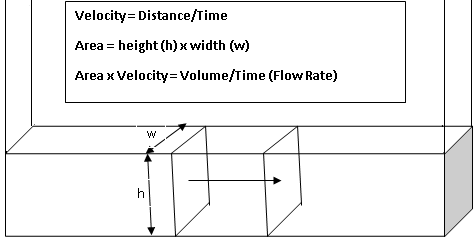
\includegraphics[scale=0.5]{ChannelFlow3}
\end{center}
$Flow (Q) = Velocity (V) * Area (A)$\\
$\implies 14 \dfrac{MG}{day}* \dfrac{10^6 gal}{MG} * \dfrac{ft^3}{7.48 gal}*\dfrac{day}{24*60*60} = V \dfrac{ft}{sec}* 6 ft * 2 ft \implies 21.7 \dfrac{ft^3}{sec}= 12V\dfrac{ft^3}{sec}$\\
$\implies V \dfrac{ft}{sec}= \dfrac{21.7}{12}= \boxed{1.8\dfrac{ft}{sec}}$\\

\item Calculate the flow, in gpd, that would pass through a grit chamber 2 feet wide, at a depth of 6 inches, with a velocity of 1 ft /sec\\
Solution:\\
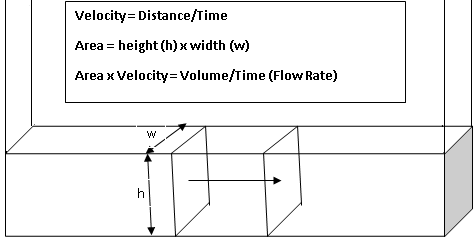
\includegraphics[scale=0.5]{ChannelFlow3}\\
$Q=V*A$\\
$Q=1\dfrac{ft}{s}*(2*0.5)ft^2=1\dfrac{ft^3}{s}$\\
$Q=1\dfrac{\cancel{ft^3}}{\cancel{s}}*\dfrac{(1440*60)\cancel{s}}{day}*7.48\dfrac{gal}{\cancel{ft^3}}=\boxed{646,272\dfrac{gal}{day}}$
\vspace{0.5cm}
\item A wastewater channel is 3.25 feet wide and is conveying a wastewater flow of 3.5 MGD. The wastewater flow is 8 inches deep. Calculate the velocity of this flow.\\
Solution:\\
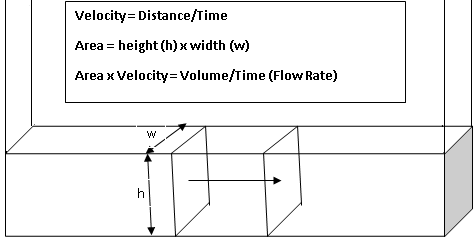
\includegraphics[scale=0.5]{ChannelFlow3}\\
$Q=V*A \implies V=\dfrac{Q}{A}$\\
$\implies V\dfrac{ft}{s}=\dfrac{3.5\dfrac{\cancel{MG}}{\cancel{day}}*\dfrac{1000000\cancel{gal}}{\cancel{MG}}*\dfrac{ft^{\cancel{3}}}{7.48\cancel{gal}}*\dfrac{\cancel{day}}{(1440*60)s}}{(3.25*0.75)\cancel{ft^2}}=\boxed{2.2\dfrac{ft}{s}}$
\vspace{0.5cm}
\item A plastic float is dropped into a wastewater channel and is found to travel 10 feet in 4.2 seconds. The channel is 2.4 feet wide and is flowing 1.8 feet deep. Calculate the flow rate of this wastewater in cubic feet per second.\\
Solution:\\
$Q=V*A$\\
$\implies Q\Big(\dfrac{ft^3}{s}\Big)=\dfrac{10ft}{4.2s}*(2.4*1.8)ft^2=\boxed{10.3\dfrac{ft^3}{s}}$
\end{enumerate}

\subsection{Grit Removal Rates}\index{Grit Removal Rates}
\emph{Typical grit removal ranges from 0.5 to 30 ft$^3$/MG}\\
\vspace{0.3cm}
\hl{Example Problems:}\\
\begin{enumerate}[1.]
\item At a wastewater treatment plant which receives a flow rate of 650,000 gallons per day, a total of 50 cubic feet of grit was removed for the month. Calculate the rate of grit removal assuming 30 days in a month.\\
Solution:\\
$Grit Removal\dfrac{ft^3}{MG}=50\dfrac{ft^3}{ \cancel{month}}*\dfrac{\cancel{month}}{30\cancel{days}}*\dfrac{\cancel{day}}{650,000\cancel{gal}}*1,000,000\dfrac{\cancel{gal}}{MG}=\boxed{2.6\dfrac{ft^3}{MG}}$
\end{enumerate}

\section{Primary Treatment} \index{Primary Treatment}
\subsection{Hydraulic or Surface Loading Rate}\index{Hydraulic or Surface Loading Rate}

The hydraulic or surface loading rate measures how rapidly wastewater moves through the primary clarifier.  It is measured in terms of the number of gallons flowing each day through one square foot surface area of the clarifier. 
$$Clarifier \enspace hydraulic \enspace loading \enspace 	\Big(\dfrac{gpd}{ft^2}\Big) =\dfrac{Clarifier \enspace influent 	\enspace flow (gpd)}{Clarifier \enspace surface \enspace area 	(ft^2)}$$ 
		Rectangular clarifier surface area  = width * length\\
		Circular clarifier surface area  = 0.785 * Diameter$^2 $\\
\subsection{Detention Time}\index{Detention Time}

Detention time is the length of time that wastewater stays in the settling tank is called the detention time.  It is also the time it takes for a unit volume of wastewater to pass entirely through a primary clarifier\\
$$Clarifier \enspace detention \enspace time \enspace (hr) = 	\dfrac{ Clarifier \enspace volume (cu.ft \enspace or \enspace gal)}{Influent \enspace flow \enspace (cu.ft \enspace or \enspace gal)/hr)}$$
Rectangular clarifier volume = width * length * depth of water\\
Circular clarifier volume = 0.785 * Diameter$^2$ * depth of water\\
Typically volume is calculated in cu. ft and influent flow is given in gallons.  Use 7.48 gal/ft$^3$ conversion factor to convert volume in cu. ft to gallons.\\

\subsection{Weir Overflow Rate}\index{Weir Overflow Rate}
The weirs at the end of the primary clarifier allow for the even distribution of the the outlet flow across the entire length of the weir.  An adequate length of weir is needed to ensure smooth and even flow of wastewater over the weirs.  Weir overflow rate measures the number of gallons of wastewater per day flowing over one foot of weir. 

		$$Weir \enspace over \enspace flow \enspace rate \Big(\dfrac{gpd}{ft}\Big) =\Big(\dfrac{Clarifier \enspace influent \enspace  flow (gpd)}{Total \enspace effluent 					\enspace weir \enspace length \enspace (ft)}\Big)$$
		Circular clarifier weir length = 3.14 * Diameter\\

\hl{Example problem for (a), (b) and (c) above:}\\
		\vspace{0.2cm}
A circular clarifier receives a flow of 11 MGD.  If the clarifier is 90 ft. in diameter and is 12 ft. deep, what is: a) the hydraulic/surface loading rate, b) clarifier detention time in hours, and c) weir overflow rate?\\
		\vspace{0.2cm}
a) Hydraulic/surface loading rate:\\
$Clarifier \enspace hydraulic \enspace loading \enspace 	\Big(\dfrac{gpd}{ft^2}\Big) ==\dfrac{\dfrac{11\cancel{MG}}{{day}}*\dfrac{10^6gal}{\cancel{MG}}}{0.785*90^2 ft^2}=\boxed{1,730gpd/ft^2}$\\
		\vspace{0.5cm}
b) Clarifier detention time:\\
$Clarifier \enspace detention \enspace time \enspace (hr) = 	\dfrac{ Clarifier \enspace volume (cu.ft \enspace or \enspace gal)}{Influent \enspace flow \enspace (cu.ft \enspace or \enspace gal)/hr)}$\\
		\vspace{0.2cm}
$Clarifier \enspace detention \enspace time \enspace (hr) = 	\dfrac{(0.785*90^2*12)\cancel{ft^3}}{\dfrac{11\cancel{MG}}{\cancel{day}}*\dfrac{10^6\cancel{gal}}{\cancel{MG}}*\dfrac{\cancel{ft^3}}{7.48\cancel{gal}}*\dfrac{\cancel{day}}{24hrs}}=\boxed{1.2hrs}$\\
		\vspace{0.5cm}
c) Weir overflow rate:\\
		\vspace{0.2cm} 
$Weir \enspace overflow \enspace rate \Big(\dfrac{gpd}{ft}\Big) =\dfrac{\dfrac{11\cancel{MG}}{{day}}*\dfrac{10^6gal}{\cancel{MG}}}{3.14*90 ft}=\boxed{38,924gpd/ft}$\\

\subsection{Removal Efficiency}\index{Removal Efficiency}		
Primary sedimentation removes suspended wastewater solids which includes BOD.  The efficiency of the primary is established as the percentage of the amount of parameter removed.  The parameter may quantified as mass (lbs) or as concentration (mg/l).

$$Removal \enspace efficiency (\%) = \dfrac{Parameter  \enspace In - Parameter  \enspace Out}{Parameter \enspace In} * 100$$

For TSS removal:\\
$$TSS \enspace Removal \enspace efficiency (\%) = \dfrac{TSS  _{In} \enspace(mg/l)  - TSS_{Out} \enspace(mg/l)  }{TSS _{In} \enspace(mg/l)  } * 100$$

For BOD removal:\\
$$BOD \enspace Removal \enspace efficiency (\%) = \dfrac{BOD_{In} \enspace(mg/l)  - BOD_{Out} \enspace(mg/l)  }{BOD _{In} \enspace(mg/l)  } * 100$$
\subsection{Solids Removal}\index{Solids Removal}	

\hl{\textbf{Type 1 Problems:}  These involve calculating lbs of solids removed given any two of the following TSS parameters - inlet concentration, outlet concentration and removal efficiency.}\\
a. If the inlet and outlet concentrations are given, calculate the mg/l of TSS removed using: 
$$TSS_{removed} = TSS_{in}(mg/l) - TSS_{out} (mg/l) $$
Then knowing the flow, use the lbs formula to calculate the lbs solids removed.

b. If either inlet or outlet concentration is given along with the clarifier removal efficiency, using the removal efficiency calculate the unknown outlet concentration (if only the inlet is given) or the inlet concentration (if only the outlet is given)\\
i) If inlet and removal efficiency is given, calculate the outlet by subtracting the product of inlet and removal efficiency from the inlet.
$$TSS_{out}=TSS_{in} - (TSS_{in}*\%Removal)$$
Example if the removal efficiency is 60\% and the inlet concentration is 300mg/l: $$TSS_{out}=300 - 300*0.6=120mg/l$$
ii) If outlet and removal efficiency is given, calculate the inlet concentration by dividing the outlet by (1-removal efficiency).\\
$$TSS_{in}=\dfrac{TSS_{out}}{1-\%Removal}$$
Example if the removal efficiency is 60\% and the outlet concentration is 120mg/l: $$TSS_{in}=\dfrac{120}{1-0.6}=300mg/l$$ 

Note:  You may derive the above formulas by algebraically manipulating: $\%Removal=\dfrac{TSS_{in} -TSS_{out}}{TSS_{in}}$\\
\hl{Example Problem:}\\
How many lbs of solids are removed daily by a primary clarifier treating a 6 MGD flow if the average influent TSS concentration is 300 mg/l and the clarifier TSS removal efficiency is 67\%.\\
$TSS_{out}=(300mg/l - 300*0.67)=99mg/l$\\
$lbs \enspace solids \enspace  removed = (300-99)mg/l*8.34*6MGD=\boxed{10,058 \enspace lbs \enspace solids \enspace removed \enspace per \enspace day}$\\
\vspace{0.5cm}
\hl{\textbf{Type 2 Problems:}  These involve calculating the amount of sludge pumping given the solids removed.  The solids removed from the primary clarifier is sludge with a typical solids concentration of about 3\% to 5\%.}\\
Given the amount of total solids removed and given the sludge concentration, the volume of sludge pumping can be calculated as follows:  $$\dfrac{ft^3\enspace sludge\enspace pumped}{ day}= \dfrac{lbs \enspace solids \enspace (removed)}{day} * \dfrac{1 \enspace lb \enspace sludge}{(\%)\enspace lbs \enspace solids}*\dfrac{gal \enspace sludge}{8.34lb \enspace sludge}*\dfrac{ft^3 \enspace sludge}{7.48 \enspace gal} $$
So for the solids removed in the above example, if the primary sludge has 5\% solids, the required sludge pumping can be calculated as:
$$\dfrac{ft^3\enspace sludge}{day}= \dfrac{10,058 \enspace \cancel{lbs \enspace solids}}{day} * \dfrac{1 \enspace \cancel{lb \enspace sludge}}{0.05\enspace \cancel{lbs \enspace solids}}*\dfrac{\cancel{gal \enspace sludge}}{8.34\cancel{lb \enspace sludge}}*\dfrac{ft^3 \enspace sludge}{7.48 \enspace \cancel{gal}}=\boxed{3,224\dfrac{ft^3 \enspace sludge}{day}} $$


\section{Trickling Filter Calculations}\index{Trickling Filter Calculations}

Trickling filter problems involve calculation of the following:

\subsection{Hydraulic or surface loading}\index{Hydraulic or surface loading}

\begin{itemize}
\item Hydraulic or surface loading is expressed as gpd/$ft^2$
\item \hl{The gpd is the total flow (Q$_T$)to the filter - primary influent flow + recirculated flow(Q$_T$= Q$_I$ + Q$_R$)}\\
\end{itemize}
			\hl{Example Problem:}\\
The total influent flow (including recirculation) to a trickling filter is 1.89 MGD. If the trickling filter is 80 ft in diameter, what is the hydraulic loading in gpd/sq ft on the trickling filter?\\
\vspace{0.2cm}
Solution:\\
\vspace{0.2cm}
$Hydraulic \enspace loading \enspace \dfrac{gpd}{ft^2}=\dfrac{(1.89*10^6)gpd}{(0.785*80^2)ft^2} =\boxed{376\dfrac{gpd}{ft^2}}$
			
			
\subsection{BOD and TSS Removal}\index{BOD and TSS Removal}
BOD and  removal is based upon the TF influent and effluent concentrations.\\
\vspace{0.2cm}
$\% Removal=\dfrac{In_{conc}-Out_{conc}}{In_{conc}}*100$\\
			\hl{Example Problem:}\\
The suspended solids concentration entering a trickling filter is 236 mg/l. If the suspended solids concentration of the trickling filter effluent is 33 mg/l, what is the suspended solids removal efficiency of the trickling filter?\\
\vspace{0.2cm}
Solution:\\
\vspace{0.2cm}
$\% Removal=\dfrac{236 mg/l-33 mg/l}{236 mg/l}*100=\boxed{86\%}$

\subsection{Organic Loading}\index{Organic Loading}

			\begin{itemize}
\item Organic loading to a trickling filter is typically expressed as lbs BOD/(day-1000 cu ft).  \item The lbs/day BOD value is the BOD loading from the primary effluent.
\item The 1000 ct. ft is the volume of the media.  
\item The media volume is calculated by multiplying the TF surface area by the media height.  
\item As the dimensions are typically given in ft., calculate the volume in $ft^3$ and then divide the calculated volume by 1000 to give the volume in units of 1000$ft^3$\\
\end{itemize}
\hl{Example Problem:}\\
A trickling filter, 70 ft in diameter with a media depth of 6 ft, receives a flow of 0.78 MGD. If the BOD concentration of the primary effluent is 167 mg/L, what is the organic loading on the trickling filter in lbs BOD/day/1000 cu ft?\\
Solution:  $Organic \enspace loading:\dfrac{lbs \enspace BOD}{day-1000ft^3}=\dfrac{lbs \enspace BOD \enspace feed \enspace to \enspace TF \enspace per \enspace day}{volume \enspace in \enspace 1000ft^3}$\\
$=\dfrac{\dfrac{(0.78*167*8.34)lbs \enspace BOD}{day}}{(0.785*70^2*6)ft^3*\dfrac{1000ft^3}{1000ft^3}}=\boxed{\dfrac{47 lbs \enspace BOD}{day-1000 ft^3}}$

\subsection{Recirculation Ratio}\index{Recirculation Ratio}


$Recirculation \enspace Ratio (R_R)=\dfrac{Recirculated \enspace Flow (Q_R)}{Influent  \enspace  Flow (Q_I)}$\\
\vspace{0.5cm}
$Recirculation \enspace Ratio (R_R)=\dfrac{Total \enspace Flow (Q_T) - Influent \enspace Flow (Q_I)}{Influent  \enspace  Flow (Q_I)}$\\
\vspace{0.5cm}
$Total \enspace Flow (Q_T) = Influent \enspace Flow (Q_I)*(Recirculation \enspace Ratio(R_R) +1)$
Make sure $Q_R$, $Q_T$ and $Q_I$ units are the same in a given problem

\hl{Example Problems:}\\
\begin{enumerate}
\item The influent to the trickling filter is 1.61 MGD. If the recirculated flow is 2.27 MGD, what is the recirculation ratio?\\
\vspace{0.2cm}
Solution:  $R_R=\dfrac{Q_R}{Q_I}=\dfrac{2.27}{1.61}=\boxed{1.4}$\\
\vspace{0.2cm}
\item A trickling filter has a total flow of 32 MGD.  If the recirculation ratio is 0.8, what is the primary effluent flow to the TF?\\
\vspace{0.2cm}
Solution:\\
\vspace{0.2cm}
$Total \enspace Flow (Q_T) = Influent \enspace Flow (Q_I)*(Recirculation \enspace Ratio(R_R) +1)$\\
$\implies 32 MGD=Q_I*(0.8+1)\implies Q_I=\dfrac{32}{1.8}=\boxed{17.8 MGD}$
\end{enumerate}




\section{Stabilization Pond Calculations} \index{Stabilization Pond Calculations}
\subsection{Pond Area}\index{Pond Area}

Formula: \hl{$Pond \enspace Area=Width * Length$}\\
\vspace{0.2cm}
also,     \hl{$Pond \enspace Area=\dfrac{Pond \enspace Volume}{Pond \enspace Depth}$}\\
\vspace{0.2cm}
\hl{Example Problem:}\\
A pond is 260 ft. long and 80 ft. wide. What is the area of this pond in acres?\\ 
\vspace{0.2cm}
Solution:\\
\vspace{0.2cm}
$(260*80)ft^2*\dfrac{acre}{43,560ft^2}=\boxed{0.48acre}$

\subsection{Solids Loading Rate}\index{Solids Loading Rate}


Formula: \hl{$Pond \enspace TSS \enspace loading \enspace rate =  \dfrac{lbs \enspace TSS}{day}$}  \\
\vspace{0.3cm}
\hl{Example Problem:}\\
\vspace{0.3cm}

The influent flow to a pond is 10,000 gallons/hour with a suspended solids concentration of 142mg/L in the raw wastewater.  How many lbs of suspended solids are sent to the pond daily?
\\
Solution:\\
\vspace{0.3cm}
$\dfrac{lbs \enspace TSS}{day}=10,000\dfrac{gal}{hr}*\dfrac{24hrs}{day}*\dfrac{MG}{1,000,000gal}*142\dfrac{mg}{l}*8.34=\boxed{284\dfrac{lbs \enspace TSS}{day}}$

\vspace{0.3cm}

\subsection{Organic Loading Rate}\index{Organic Loading Rate}

\vspace{0.3cm}
Formula: \hl{$Pond \enspace organic \enspace loading \enspace rate =  \dfrac{lbs \enspace BOD/day}{Area (acre)}$}  \\
\vspace{0.3cm}
\hl{Example Problem:}\\
\vspace{0.3cm}
The flow to a pond is 7.2MGD. If the pond diameter is 350 ft and the BOD in the pond influent is 170mg/L, what is the organic loading to this pond in lbs BOD/day/acre?
\\
Solution:\\
\vspace{0.3cm}
$Organic \enspace loading=\dfrac{lbs \enspace BOD \enspace per \enspace day}{area \enspace (acres)}=\dfrac{(7.2MGD \enspace * \enspace 170mg/l \enspace * \enspace 8.34)}{0.785*350^2ft^2}*\dfrac{43,560ft^2}{acre}=\boxed{\dfrac{4,624lbs \enspace BOD}{day-acre}}$

\vspace{0.3cm}

\subsection{Detention time}\index{Detention time}
\vspace{0.3cm}
Formula: \hl{$Pond \enspace detention \enspace time=\dfrac{Volume}{Flow}$}\\ 
\vspace{0.3cm}
\hl{Example Problem:}\\
A 40 acre wastewater treatment pond receives a flow of 0.6 MGD. If the pond is operated at a depth of 4ft. What is the detention time of this pond?\\
Solution:\\
$Pond \enspace detention \enspace time=\dfrac{Volume}{Flow}=\dfrac{(40*4)acre-ft}{0.6*10^6\dfrac{gal}{day}*\dfrac{ft^3}{7.48gal}*\dfrac{acre-ft}{43,560ft^3}}=\boxed{87 \enspace days}$\\
\vspace{0.3cm}


\subsection{Hydraulic Loading Rate}\index{Hydraulic Loading Rate}
Formula:\hl{$Pond \enspace hydraulic \enspace loading \enspace rate \enspace \Bigg[\dfrac{in}{day}\Bigg]=\dfrac{Flow}{Area}$}\\
also, \hl{$Pond \enspace hydraulic \enspace loading \enspace rate \Bigg[\dfrac{in}{day}\Bigg]=\dfrac{Pond \enspace depth \enspace (in)}{Pond \enspace detention  \enspace time \enspace \dfrac{Volume}{Flow}}$ }\\
The second formula above is because:\\
\vspace{0.3cm}
$Hydraulic \enspace Loading \enspace (HL)=\dfrac{Flow}{Area}$\\
\vspace{0.3cm}
$Detention \enspace time \enspace (DT)=\dfrac{Vol}{Flow} \implies Flow=\dfrac{Vol}{DT} $\\
\vspace{0.3cm}
Substituting for flow in  the HL formula above:\\
\vspace{0.3cm}
$HL=\dfrac{\dfrac{Vol}{DT}}{Area}\enspace or \enspace \dfrac{Vol}{Area*DT} \enspace \implies \boxed{HL=\dfrac{Pond \enspace Depth}{DT}} \enspace as \enspace \dfrac{Vol}{Area}=Pond \enspace Depth$\\
\vspace{0.3cm}
\textbf{Example Problems:}\\
\begin{enumerate}

\item Find hydraulic loading in inches/day for a pond given the following:
\begin{itemize}
\item Pond depth = 12ft.
\item Pond volume = 1,400,000ft3
\item Pond flow = 1,000,000gal/day
\end{itemize}
Solution:\\
$Pond \enspace hydraulic \enspace loading \enspace rate \enspace \Bigg[\dfrac{in}{day}\Bigg]=\dfrac{Flow}{Area}$\\
$ \implies\dfrac{1,000,000\dfrac{gal}{day}*\dfrac{ft^3 }{7.48gal}}{\dfrac{1,400,000ft^3}{12ft}}*12\dfrac{in}{ft}=\boxed{13.8\dfrac{in}{day}}$\\
\vspace{0.3cm}
\hl{Note:  The area of the pond was found by dividing the volume (1,000,000$ft^3$) by the pond depth (12ft)}
\vspace{0.3cm}

\item Find pond hydraulic loading in inches/day when the depth of the pond is 6 ft. and the detention time is 30 days.\\
Solution:\\



$Pond \enspace hydraulic \enspace loading \enspace rate=\dfrac{Pond \enspace depth \enspace (in)}{Pond \enspace detention  \enspace time \enspace \dfrac{Volume}{Flow}}$\\
$\implies \dfrac{6*12 \enspace inches}{30 \enspace days}=\boxed{\dfrac{2.4in}{day}}$
\end{enumerate}


\section{Activated Sludge Calculations} \index{Activated Sludge Calculations}
\subsection{Mean Cell Residence Time}\index{Mean Cell Residence Time}


The MCRT is calculated as:\\  
\vspace{0.2cm}
$MCRT(days) = $\\
$\dfrac{Total \enspace MLSS \enspace lbs \enspace in \enspace the \enspace aeration \enspace system \enspace (aeration \enspace tank \enspace + \enspace clarifier)}{Total \enspace amount \enspace in \enspace lbs/day \enspace of \enspace suspended \enspace solids \enspace leaving  \enspace the \enspace system \enspace(Effluent\enspace SS+ WAS \enspace solids)}$\\
\vspace{0.4cm} 
$MCRT (days) = \dfrac{MLSS \enspace in \enspace aeration \enspace tank \enspace (lbs)+MLSS \enspace in \enspace clarifier \enspace (lbs)}{Effluent \enspace suspended \enspace solids \enspace (lbs/day)+\enspace WAS \enspace SS \enspace (lbs/day)}$\\
\vspace{0.3cm}
\textbf{Key Points for Solving MCRT Problems}\\
\begin{enumerate}
\item \textbf{MLSS quantification}:\\ 
\begin{itemize}
\item Pounds formula is used to calculate lbs MLSS using: i) aeration tank and the clarifier volumes, and ii) the given MLSS concentration.  
\item The MLSS concentrations for the aeration tank and the clarifier are the same.  So the given MLSS concentration applies to both - the aeration tank and the clarifier
\item Make sure it is the MLSS concentration that you are using not the MLVSS concentration.  
\item If MLSS concentration is not given but instead MLVSS concentration is given, you will need to find the MLSS concentration by dividing the MLVSS conc. by the mixed liquor volatile solids, as MLVSS(conc.) = MLSS * \% volatile solids
\end{itemize}

\item \textbf{Suspended solids quantification}:\\ 
\begin{enumerate}
\item \textbf{Effluent suspended solids}
\begin{itemize}
\item Effluent suspended solids can be quantified using the pounds formula - using the effluent flow (in MGD) and the effluent suspended solids concentration.
\end{itemize}
\item \textbf{WAS suspended solids}
\begin{itemize}
\item Use pounds formula given the WAS flow (make sure it is in MG) and the WAS SS concentration
\item Note that the WAS and RAS streams have the same SS concentration.  If WAS SS concentration is not specified, use the RAS SS concentration
\end{itemize}
\end{enumerate}
\end{enumerate} 

\hl{Example Problems:}\\
\begin{enumerate}
\item In an conventional activated sludge plant  the aeration tank contains 6000 lbs of MLSS and the final clarifier contains 2300 lbs of MLSS. 1450 lbs of solids are wasted each day and 90 lbs/day of solids leave in the final effluent. Calculate the MCRT for this plant.\\
Solution:\\
\vspace{0.2cm} 
$MCRT (days) =  \dfrac{MLSS \enspace in \enspace aeration \enspace tank \enspace (lbs)+MLSS \enspace in \enspace clarifier \enspace (lbs)}{SS \enspace effluent \enspace (lbs/day)+SS \enspace WAS \enspace (lbs/day)}$\\
\vspace{0.2cm} 
$MCRT (days) =  \dfrac{6000lbs \enspace + \enspace 2300 lbs}{90lbs/day\enspace + \enspace 1450 lbs/day}=5.4=\boxed{5days}$\\
\vspace{0.3cm} 
\item A activated sludge plant treats an average influent flow of 4 MGD.  The plant has two  aeration tanks – 0.45 MG volume each and two final clarifiers – 0.2 MG volume each, and a mixed liquor suspended solids concentration averages  1800 mg/l.   The effluent suspended solids concentration averages 18 mg/L. The WAS flow is 100,000 gallons per day has a SS concentration of 6100 mg/L. Calculate the MCRT\\
Solution:\\
$MCRT (days) =  \dfrac{MLSS \enspace in \enspace aeration \enspace tank \enspace (lbs)+MLSS \enspace in \enspace clarifier \enspace (lbs)}{SS \enspace effluent \enspace (lbs/day)+SS \enspace WAS \enspace (lbs/day)}$\\
\vspace{0.3cm} 
$MLSS \enspace in \enspace aeration \enspace tank \enspace (lbs)=2*0.45*1800*8.34=13511lbs$\\
\vspace{0.3cm} 
$MLSS \enspace in \enspace clarifier \enspace (lbs)=2*0.2*1800*8.34=6005lbs$\\
\vspace{0.3cm} 
$SS \enspace effluent \enspace (lbs/day)=4MGD *18mg/l*8.34=600lbs/day$\\
\vspace{0.3cm} 
$SS \enspace WAS \enspace (lbs/day)=\dfrac{100000}{1000000}MGD *4800mg/l*8.34=4003lbs/day$\\
\vspace{0.3cm} 
Plugging in the values calculated above: $MCRT (days) =  \dfrac{13511+6005}{600+4003}=4.2=\boxed{4days}$\\
\end{enumerate}

\subsection{F:M (Food to Microorganism Ratio}\index{F:M (Food to Microorganism Ratio}

\begin{itemize}
\item This parameter ratios the food – the mass of primary effluent BOD entering the aeration basin to the mass of the microorganisms - \textbf{MLVSS}, in the aeration basin.
\item \textbf{Only the mass of the microorganisms (MLVSS) in the aeration basin is used – the mass of microorganisms in the secondary clarifier is not considered}
\item Common ranges for F/M for a conventional activated sludge plant are from 0.15 to 0.5. 
\item The optimum F/M varies from plant to plant and can be determined by trial and error.
\item The F:M may be used to determine the concentration of mixed liquor suspended solids to be maintained in the aeration tank.
\item Generally, low F/M ratios should be carried during the colder months as the microorganism activity (metabolism) is lower.
\item F:M and MCRT are inversely related: that is a long MCRT means a low F:M and a short MCRT means a high F:M
\end{itemize}
F:M=$\dfrac{amount \enspace of \enspace food \enspace coming \enspace in}{amount \enspace of \enspace microorganisms \enspace present}$\\
\vspace{0.3cm}
\hspace{0.7cm}$=\dfrac{(lbs/day) \enspace primary \enspace effluent  \enspace BOD \enspace entering \enspace the  \enspace aeration \enspace tank}{(lbs) \enspace MLVSS \enspace in \enspace the  \enspace aeration \enspace tank}$\\
\vspace{0.3cm}
\textbf{Key Points for Solving F:M Problem}\\
\begin{enumerate}
\item \textbf{Quantifying F:}
\begin{itemize}
\item use the pounds formula to calculate the lbs/day of BOD in the primary effluent.\\
lbs/day BOD = Primary eff. flow (MGD)* Primary eff. BOD concentration (mg/l) * 8.34\\
\end{itemize}
\item \textbf{Quantifying M:}
\begin{itemize}
\item The concentration of the microorganisms is assumed to be the same as the MLVSS concentration
\item \textbf{Only the mass of the microorganisms (MLVSS) in the aeration basin is used – the mass of microorganisms in the secondary clarifier is not considered} 
\item lbs MLVSS may be calculated using pounds formula using the volume of the aeration tank (in MG) and the MLVSS concentration
\item If the MLVSS concentration is not given, it can be calculated from the MLSS and MLSS \% volatile matter (solids) concentration\\
MLVSS = MLSS * \% MLSS volatile solids
\end{itemize}


\hl{Example Problem:}\\
\begin{enumerate}[i.]
\item A conventional activated sludge plant receives an average flow of 5.5 MGD. The influent BOD to the plant averages 230mg/l and the primary effluent BOD average 160 mg/l. The 1 MG aeration tank has an MLSS concentration of 2800 mg/L and the MLVSS volatile solids content is 75\%. Calculated the F:M ratio for this plant.
\vspace{0.3cm}
Solution:\\
\vspace{0.3cm}
F=5.5*160*8.34=7339lbs/day BOD\\
M=1*2800*0.75*8.34=17514lbs MLVSS\\
F:M=$\dfrac{7339}{17514}=\boxed{0.41}$\\

Note:  The 160 mg/l BOD concentration of the primary effluent was used for the F calculation and not 230mg/l - which is the BOD concentration of the flow coming into the plant\\
\end{enumerate}


\subsection{Sludge Volume Index (SVI)}\index{Sludge Volume Index (SVI)}

\begin{itemize}
\item SVI measures the settleability and compactibility of the secondary sludge
\item It is calculated using results from the 30-minute settleability test and the MLSS concentration
\item SVI is expressed in ml/g and it is essentially the volume (ml) of 1 gram of the MLSS after 30 minutes of settling
\item it provides a more accurate picture of the sludge settling characteristics than settleability or MLSS alone
\item 50 to 120 ml/gm SVI value is considered
optimal. Higher SVI values indicate sludge that is slow to settle and not compacting well. When SVI
values are approaching 200 ml/gm, activated sludge process is considered to be "bulking".
\end{itemize}
\end{enumerate}
SVI (ml/g)= $\dfrac{Settled \enspace sludge \enspace volume \enspace in \enspace ml/l \enspace after \enspace 30 \enspace min}{MLSS \enspace mg/l}*1000 \dfrac{mg}{g}$\\
\vspace{0.3cm}
\textbf{Key Points for Solving SVI Problems}\\
\begin{itemize}
\item For the settling test MLSS is typically settled in a 1 liter settleometer.  The volume of the settled solids is therefore read as ml/L.  So if for any reason a larger or smaller volume of the mixed liquor sample is taken, the settle solids value should commensurate with the volume of the MLSS sample.  For example, if a 2 liter settleometer is used and if the solids settle to 400 ml in that settleometer, the ml/L will be 400ml/2L or 200ml/L
\item For some problems, the settled solids volume is provided as a percentage (\%).  So if a 1-liter settlometer is used and the settled solids volume is reported as 25\%, it implies a settled sludge volume of 250ml/L
\end{itemize} 
\hl{Example Problem:}\\
\begin{enumerate}[i.]
\item In an aeration tank, the MLSS is 2500 mg/l and recorded 30-minute settling test indicates 230 ml/L.  What is the sludge volume index?\\
\vspace{0.3cm}
Solution:\\
SVI=$\dfrac{230ml/l}{2500mg/l}*1000\dfrac{mg}{g}=\boxed{92ml/g}$
\end{enumerate}

\subsection{Sample Math Problems}\index{Sample Math Problems}

\begin{enumerate}

\item An activated sludge plant operates well at an F:M ratio of between 0.23 and 0.28.  Calculate the minimum MLSS concentration, given the following:\\
Q = 0.4 MGD\\
Primary influent BOD = 250 mg/l\\
Primary effluent BOD = 128 mg/l\\
Aeration tank vol. = 350,000 gallons\\
Clarifier vol = 250,000 gallons\\
MLSS has 80\% volatile solids\\
\vspace{0.3cm}
Solution:\\
\vspace{0.3cm}
$F:M=\dfrac{(lbs/day) \enspace primary \enspace effluent  \enspace BOD \enspace entering \enspace the  \enspace aeration \enspace tank}{(lbs) \enspace MLVSS \enspace in \enspace the  \enspace aeration \enspace tank}$\\
\vspace{0.3cm}
$\implies F:M \propto \dfrac{1}{MLSS \enspace concentration}$  $\implies$ F:M is inversely proportional to MLSS\\
\vspace{0.3cm}
So to have minimum MLSS conc. F:M needs to be the maximum of the range provided\\
\vspace{0.3cm}
If the MLSS concentration = x:
$ \implies F:M=0.28=\dfrac{0.4*128*8.34}{0.35*x*0.8}\implies x = \boxed{5,446 mg/l \enspace MLSS}$


\newpage

\item Given that an activated sludge plant with an influent flow of 1.2 MGD is operated at an MCRT of 6 days and the parameters below, calculate the WAS flow rate (wasting rate) in gallon per day.
\\
\vspace{0.3cm}
Solution:\\
\vspace{0.3cm}
\renewcommand{\arraystretch}{1.6}
\begin{tabular}{ | m {7 cm} | m {7 cm}| } 
 \hline
Two aeration tanks – 0.5 MG each & Two final clarifiers – 0.25 MG each \\ 
 \hline
 Final effluent $= 20\dfrac{mg}{l}$ & WAS – 7500 ppm\\ 
 \hline
 MLSS –$3600\dfrac{mg}{L}$ & MLSS volatile solids content = 80\%  \\
 \hline
\end{tabular}
\\
\vspace{0.3cm}
$ MCRT \enspace =\dfrac{lbs \enspace MLSS (system)}{\dfrac{lbs}{day} \enspace Effluent_{SS} + \dfrac{lbs}{day} \enspace WAS_{SS}}  $
\\
\vspace{0.3cm}
\noindent \textbf{Step 1:  Calculate the lbs MLSS (system):}\\
\vspace{0.3cm}
\noindent $lbs \enspace MLSS \enspace (system) \enspace =(2*0.5 + 2*0.25)MG * 3,600\dfrac{mg}{L} * 8.34 = 45,036 \enspace lbs$
\\
\vspace{0.3cm}
\noindent \textbf{Step 2:  Calculate the lbs/day Effluent$_{SS}$:}\\
\vspace{0.3cm}
\noindent $\dfrac{lbs}{day} \enspace Effluent_{SS}= 1.2 MG * 20\dfrac{mg}{L} * 8.34 = 200.2lbs$
\\
\vspace{0.3cm}
\noindent \textbf{Step 3:  Plug in the values in the MCRT formula:}\\
\vspace{0.3cm}
\noindent MCRT: $6 \enspace days=\dfrac{45,036}{200.2 \dfrac{lbs}{day}+ \dfrac{lbs}{day}WAS_{SS}}  $
\\
\vspace{0.3cm}
\noindent \textbf{Step 4:  Solving for WAS$_{SS}$:}\\
\vspace{0.3cm}
\noindent $\dfrac{lbs}{day}WAS_{SS} = \dfrac{45,036}{6} - 200.2 = 7,306 \dfrac{lbs}{day}$
\\
\vspace{0.3cm}
\noindent \textbf{Step 5:  Solving for WAS flow using the lbs formula:}\\
\vspace{0.3cm}
\noindent $7,306 \dfrac{lbs}{day} = WAS \enspace Flow \enspace (MGD) * 7,500 * 8.34$\\
\vspace{0.3cm}
\noindent $ \implies WAS \enspace Flow \enspace (MGD)=\dfrac{7,306}{7,500*8.34}=0.116 MGD = \boxed {116,000 \enspace \dfrac{gal}{day}}  $



\end{enumerate}








\section{Solids Thickening Calculations} \index{Solids Thickening Calculations}

\begin{enumerate}
\item Calculate the air required (SCFM) to meet a 0.04 lb air:lb feed solids ratio for a 100 GPM WAS flow
with a solids content of 6500mg/l? Assume 0.08 lbs air/SCF air.
Solution:
$$\dfrac{lb \enspace air}{lb \enspace solids}=0.04=\dfrac{0.08 \enspace lbs \enspace air \enspace SCF * X \enspace SCF \enspace per \enspace minute}{\dfrac{100}{1,000,000}\dfrac{MG}{min}*6,500\dfrac{mg}{l}*8.34 \enspace lbs \enspace solids}$$

$$\implies x \enspace SCF \enspace per \enspace minute = \dfrac{0.04*5.421}{0.08}=\boxed{2.7 \enspace SCFM}$$

\item A treatment plant receives an influent flow of 30 MGD with a TSS concentration of 280 mg/l.  The primary treatment removes 55\% TS and the primary sludge is pumped to a 40 ft diameter gravity thickener.  Calculate the average solids loading to the thickener in lbs TSS/day-ft$^2$\\
Solution:\\
 
Solids loading to gravity thickener=$\dfrac{(30 \enspace MGD \enspace * \enspace 280*0.55 \enspace mg/l \enspace *8.34) lbs \enspace TSS \enspace per  \enspace day}{0.785*40^2 \enspace ft^2}=\boxed{30.7 \enspace lbs \enspace TSS/day-ft^2}$

\end{enumerate}



\section{Digester Calculations}\index{Digester Calculations}
\subsection{Sludge Pumping}\index{Sludge Pumping}
			
				\hl{Example Problems:}\\
					\begin{enumerate}
						\item A primary clarifier receives an average flow of 12 MGD containing 280mg/L of TSS.  This clarifier typically removes 75\% TSS  and produces a 3.5\% sludge and the sludge pump is rated to pump 35 cu.ft/min.
							\begin{enumerate}[a.]
								\item How many pounds of TSS is removed in the clarifier?

								\item How many cu.ft of sludge at the given 3.5\% sludge needs to be pumped per day to remove the solids?

								\item How many minutes would the sludge pump need to be operational each day to pump the required amount of sludge - calculated from ii.  above?

								\item For how many minutes each hour the sludge pump should be programmed to operate (Given the number of minutes the pump need to operate per day calculated from iii. above) ?\\
							\end{enumerate}
						Solution:\\
							\begin{enumerate}[a.]
								\item $lbs \enspace solids \enspace removed=(280*0.75)mg/l*12MGD*8.34=\boxed{21,017 \enspace lbs \enspace solids \enspace per \enspace day}$\\
								\vspace{0.5cm}
								\item $\dfrac{21,017 \enspace lbs \enspace solids}{day} = \dfrac{x \enspace \cancel{ft^3\enspace sludge}}{day} *\dfrac{7.48 \enspace \cancel{gal \enspace sludge}}{\cancel{ft^3 \enspace sludge}}* \dfrac{0.035 \enspace lbs \enspace solids}{1 \enspace \cancel{ {lb \enspace sludge}}}*\dfrac{8.34 \enspace \cancel{lb \enspace sludge}}{\cancel{gal \enspace sludge}}$\\
								\vspace{0.5cm}
								$\dfrac{x \enspace ft^3\enspace sludge}{day}= \dfrac{21,017}{0.035*834*7.48}=\boxed{9,626\dfrac{ft^3 \enspace sludge}{day}} $\\
								\vspace{0.5cm}
								\item $\dfrac{9,626 \enspace ft^3 \enspace sludge}{day}*\dfrac{min}{35 \enspace ft^3 \enspace sludge}=\boxed{\dfrac{275 \enspace minutes}{day}}$\\
								\vspace{0.5cm}
								\item $\dfrac{275 \enspace minutes}{day}*\dfrac{day}{24 \enspace hrs}=\boxed{\dfrac{11.4 \enspace minutes}{hr}}$\\
							\end{enumerate}
								\vspace{0.2cm}
						\item Calculate the lbs/day of solids removed in a primary clarifier treating a 5 MGD flow with an average influent and effluent TSS concentrations of 250 mg/l and 98 mg/l respectively.
						\vspace{0.2cm}
						Solution:\\
						\vspace{0.2cm}
						$\dfrac{lbs}{day}=5 MGD *(250-98)\dfrac{mg}{l}*8.34 = \boxed{6338\dfrac{lbs}{day}}$
				\end{enumerate}
				
\subsection{Sludge Blending} \index{Sludge Blending}

\begin{itemize}
\item In digestion the feed is typically a blend of primary and secondary sludges - each of which have different total and organic solids content.

\item Thus, \textbf{for blending calculations}, if:\\

C$_1$ and V$_1$ is the concentration and volume (flow) respectively of the primary sludge portion of the digester feed, and\\
 \vspace{0.2cm}
 C$_2$ and V$_2$ is the concentration and volume (flow) respectively of the secondary sludge feed 
 \vspace{0.2cm}
C$_3$ and and V$_3$ is the concentration and volume (flow) respectively of the digester sludge feed\\
\vspace{0.3cm}
The sum of the mass from each of the two source sludge feeds will equal to the mass in the digester sludge feed:\\
\vspace{0.3cm}
\textbf{C$_1$ * V$_1$ + C$_2$ * V$_2$ =  C$_3$ * V$_3$.}\\
\vspace{0.3cm}
This equation can be manipulated algebraically to calculate anyone of the unknown values in the equation.\\
\vspace{0.2cm}
Also, any of the three volume variables can be expressed as the sum or difference of the other two - , or V$_1$ + V$_2$ = V$_3$ or V$_1$ = V$_3$ - V$_2$ or V$_2$ = V$_T$ - V$_1$\\

\end{itemize}

\textbf{Example Problem:}  Two sludges are blended together as follows: 15,000 gal. primary sludge at 4.1\% solids. 28,000 gal. secondary sludge at 1.3\% solids. What is the combined solids concentration?  If the primary sludge is 68\% VS and the secondary sludge is 63\% VS, what is the VS concentration (\%) in the combined sludge?\\
\vspace{0.2cm}
Solution:\\
\vspace{0.2cm}
Combined solids concentration:\\
\vspace{0.2cm}
$
C_1*V_1 + C_2*V_2 = C_3*V_3$\\
\vspace{0.2cm}
$\implies C_3 = \dfrac{C_1*V_1 + C_2*V_2}{V3}=\dfrac{C_1*V_1 + C_2*V_2}{V_1 + V_2}=\dfrac{4.1*15,000 + 1.3*28,000}{15,000 + 28,000}=\boxed{2.28\%}
$\\
\vspace{0.2cm}
Lbs of VS in combined sludge:\\
\vspace{0.2cm}
$
C\textsubscript{VS1}*V_1 + C\textsubscript{VS2}*V_2 = C\textsubscript{VS3}*V_3$\\
\vspace{0.2cm}
$\implies C\textsubscript{VS3} = \dfrac{C\textsubscript{VS1}*V_1 + C\textsubscript{VS2}*V_2}{V3}=\dfrac{C\textsubscript{VS1}*V_1 + C\textsubscript{VS1}*V_2}{V_1 + V_2}$\\
\vspace{0.2cm}
$\implies C\textsubscript{VS3}
=\dfrac{4.1*15,000*0.68 + 1.3*28,000*0.63}{15,000 + 28,000}=\boxed{1.50\%}$
\\

\vspace{0.3cm}













				
				
\subsection{Digester VS or Organic Loading}\index{Digester VS or Organic Loading}				
				\hl{Example Problems:}\\

				\begin{enumerate}
					\item How many pounds of TS and VS are pumped to a digester each day if the digester receives 10,000 gpd of sludge at 5\% solids concentration with an average VS\% of 75\%?\\
					Solution:\\

					Digester TS loading (lbs/day)\\
					\vspace{0.3cm}
						$
							\dfrac{lbs \enspace TS}{day}
							=
							\dfrac{10,000 \enspace gal \enspace sludge}{day}
							*
							\dfrac{(8.34*0.05) lbs \enspace TS )}{gal \enspace sludge}
							=4,170
							\dfrac{lbs \enspace TS}{day}
						$
						\\
						\vspace{0.3cm}
						Digester VS loading (lbs/day)\\
						\vspace{0.3cm}
						$=4,170 	\dfrac{lbs \enspace TS}{day}*0.75\dfrac{lbs \enspace VS}{lb \enspace TS}=\boxed{3,128 \dfrac{lbs \enspace VS}{day}}$
						\vspace{0.5cm}
						\item An anaerobic digester is 37’ in diameter and 27’ deep with a 5,000 gallon daily sludge flow. The sludge is 6\% solids and 66\% volatile solids.  What is the volatile solids loading in pounds per cubic foot per day?
							
							
						Solution:\\
						{
						$
							Digester \enspace volatile \enspace solids 			\enspace loading \enspace rate = 					\dfrac
							{
							Digester \enspace Loading 
								\dfrac
								{
								lbs \enspace VS
								}
								{
								day
								}
							}
							{
							Digester \enspace volume (V)ft^3
							}
						$
						}\\
						\begin{center}
						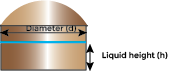
\includegraphics[scale=1]{DigesterWOCDimensions_1}
						\end{center}

						{
						$=\dfrac
							{
								5000
								\dfrac
									{gal \enspace sludge}
									{day}
								*(8.34*0.06*0.66) 
								\dfrac
									{lbs \enspace VS}
									{gal \enspace  sludge}
							}
							{
								(\dfrac
									{\pi}
									{4}*37^2*27)ft^3
							}
						=\boxed
							{
								0.057 \dfrac
									{lbs \enspace VS}
									{day-ft^3}
							}
						$}
				\end{enumerate}
\subsection{Total volatile solids (VS) reduction}\index{Total volatile solids (VS) reduction}	
				\begin{itemize}
					\item This provide a measure of the organic matter content removed and converted into digester gas in the digester. 
					\item Higher volatile solids reduction implies higher gas production and lower biosolids hauling costs.\\
					\item The VS reduction of the digester is provided by the Van Kleeck equation \\ 

					$$Digester \enspace VS \enspace reduction (\%)=\dfrac{VS_{in}-VS_{out}}{VS_{in}-VS_{in}*VS_{out}}*100$$

					\item Digester volatile solids concentration is typically expressed as a percentage of the sludge total solids.\\
					\item 70\% VS which means that 70\% of the total solids is volatile solids.
					\item \hl{The value of $VS_{in}$ and $VS_{out}$ for the digester VS reduction (Van Kleek) equation above should be in fraction and not as a percentage.}\\
					\vspace{0.2cm}
					A value of 0.7 should be used in the equation if the VS concentration is 70\%. Likewise, as 0.525 if the VS concentration is 52.5\%.\\
					\vspace{0.2cm}
					Applying this equation to calculate the digester VS reduction if the inlet sludge VS averages 75\% and the outlet sludge is 58\%?\\
					\vspace{0.3cm}
					\hl{Example Problem:}\\
					Calculate the \% VS reduction in a digester given the volatile solids content of the influent sludge to the digester is 70\% and the volatile solids content of the sludge leaving the digester is 52.5\%\\
					Solution:  $Digester \enspace VS \enspace reduction (\%)=\dfrac{0.7-0.525}{0.7-0.7*0.525}*100=\boxed{ 53\%}$\\
					\vspace{0.2cm}
				\end{itemize}



\section{Dewatering math problems}\index{Dewatering math problems}


\textbf{Solving Dewatering Problems}
\begin{enumerate}
	\item \textbf{Calculation of solids recovery}\\
		\begin{enumerate}
		\item Calculate amount of solids fed to the dewatering unit
		\item Calculate the amount of solids produced as part of the dewatered cake
		\item The ratio of the solids in dewatered cake to that in the feed times 100 will give you the solids recovery (solids recovery rate)
		\end{enumerate}
	\item \textbf{Calculation of dewatered cake volume}\\
		\begin{enumerate}
		\item First calculate the amount of cake solids produced in terms of weight per time.
		\item From the weight of the cake produced calculate the volume - from the cake density which is normally given\\
		\end{enumerate}
	\item \textbf{Calculation of solids hauling costs or savings associated with change in cake solids content}\\
		\begin{enumerate}
		\item First calculate the amount of dry solids produced as part of the original wet cake solids percent
		\item Using the value of the dry solids calculate the wet cake weight with the new cake solids percentage\\
		\end{enumerate}
	\item \textbf{General formula for calculating net savings associated with change in cake solids content}\\
Savings =$ \dfrac {(New \enspace solids \enspace \%-Old \enspace Solids \enspace \%)}{New \enspace solids \enspace \%}*Old \enspace Cost$

So if the cake dryness goes up from 20\% to 26\% and currently a utility is spending \$ 1,000,000 per year for biosolids hauling and disposal, their net savings will be: (26\%-\%20)/26*\$ 1,000,000 = \$ 230,769
\end{enumerate}

\subsection{Calculation of solids recovery}\index{Calculation of solids recovery}



                \hl{Example Problems:}\\


(a) Calculate amount of solids fed to the dewatering unit\\
(b) Calculate the amount of solids produced as part of the dewatered cake\\
(c) The ratio of the solids in dewatered cake to that in the feed times 100 will give you the solids\\
recovery (solids recovery rate)\\


\subsection{Calculation of dewatered cake volume}\index{Calculation of dewatered cake volume}

(a) First calculate the amount of cake solids produced in terms of weight per time.\\
(b) From the weight of the cake produced calculate the volume - from the cake density which is
normally given\\

\subsection{Hauling cost impact due to solids content change}\index{Hauling cost impact due to solids content change}

(a) First calculate the amount of dry solids produced as part of the original wet cake solids percent\\
(b) Using the value of the dry solids calculate the wet cake weight with the new cake solids percentage\\

General formula for calculating net savings associated with change in cake solids content:\\
\vspace{0.2cm}
$Savings = \dfrac{(New \enspace solids(\%) - Old \enspace Solids(\%)}{Old \enspace solids(\%)}*Old \enspace Cost$\\
So if the average cake dryness goes up from 20\% to 26\% and currently this utility is spending \$ 1,000,000 per
year for biosolids hauling and disposal, their net savings will be:\\
\vspace{0.2cm}
$\dfrac{(26\%-20\%)}{20\%}* 1,000,000 = \$300,000$\\
\vspace{0.2cm}
\hl{Example Problems}\\
\begin{enumerate}[1.]


\item 12,000 $ft^3$ of anaerobically digested sludge containing 2.8\% TS is dewatered in a centrifuge.  The centrifuge yields 37 $yd^3$ of 26\% of dewatered cake with a density of 73 lb/$ft^3$.  Calculate the solids capture rate.\\


 
\vspace{0.1cm}
Solution:\\
\vspace{0.1cm}
$
    lbs \enspace TS \enspace feed \enspace to \enspace centrifuge
    =
    12,000 ft^3 \enspace sludge
    *
    7.48 
    \dfrac
    {
    gal
    }
    {
    ft^3
    }
    *
    \dfrac
    {
    (8.34*0.028 lbs \enspace TS )
    }
    {gal \enspace sludge
    }
    =20,960 {lbs \enspace TS}
$
\vspace{0.2cm}
$
    lbs \enspace TS \enspace feed \enspace from \enspace centrifuge
    =
    37 yd^3 \enspace sludge
    *
    27 
    \dfrac
    {
    ft^3
    }
    {
    yd^3
    }
    *
    \dfrac
    {
    (73 lbs *0.26 \enspace TS )
    }
    {ft^3 \enspace sludge
    }
    =18,961 {lbs \enspace TS}
$
\vspace{0.2cm}
$
    solids \enspace capture \enspace rate
    =
    \dfrac
    {
    18,961 lbs \enspace solids \enspace produced        \enspace by \enspace centrifuge
    }
    {
    20,960 lbs \enspace solids \enspace fed             \enspace from \enspace digester
    }
    *
    100 
    =\boxed
    {
    90.4\% solids \enspace capture
    }
$

\vspace{0.2cm}
\item At a 60 GPM of 2.8\% feed a belt press which has a 90\% solids capture rate produces a 20\% cake at 68 lbs/$ft^3$.  How long would it take to fill a 3 $yd^3$ bin  
\vspace{0.2cm}   
    
Solution:\\
\vspace{0.2cm}
{$\dfrac{cake \enspace TS \enspace produced - lbs}{min}= \dfrac {60 gallons \enspace sludge}{min}*\dfrac {8.34 lbs \enspace sludge \enspace feed}{galllon}*\dfrac{0.028 lbs \enspace TS}{lb \enspace sludge}*0.9$}\\
\vspace{3mm}

{$=\dfrac{12.61lbs \enspace TS}{min}$}\\
\vspace{3mm}

{$\dfrac{ft^3 \enspace cake \enspace produced}{min}=\dfrac{12.61lbs \enspace TS}{min}*\dfrac{100 lbs \enspace cake}{20lbs \enspace TS}*\dfrac{ft^3 \enspace cake}{68 lbs \enspace cake} = \dfrac{0.927ft^3 cake}{min}$}\\
\vspace{3mm}

{$\dfrac{ft^3 \enspace cake \enspace produced}{min}=\dfrac{12.61lbs \enspace TS}{min}*\dfrac{100 lbs \enspace cake}{20lbs \enspace TS}*\dfrac{ft^3 \enspace cake}{68 lbs \enspace cake} = \dfrac{0.927ft^3 cake}{min}$}\\
\vspace{3mm}

{$Time \enspace required \enspace to \enspace fill \enspace the \enspace bin=\dfrac{min}{0.927ft^3}*{3yd^3}*\dfrac{27ft^3}{yd^3}=\boxed{75min}$}\\


\end{enumerate}

\section{Chlorine dosing problems}\index{Chlorine dosing problems}
\textbf{Example 1:}\\
Determine the chlorinator setting (lb/day) required to treat a flow of $4 \mathrm{MGD}$ with a chlorine dose of $5 \mathrm{mg} / \mathrm{L}$.

Chlorine feed rate $(\mathrm{lb} /$ day $)=$ Chlorine $(\mathrm{mg} / \mathrm{L}) \times$ Flow $(\mathrm{MGD}) \times 8.34 \mathrm{lb} / \mathrm{gal}$

Chlorine feed rate $(\mathrm{lb} /$ day $)=5 \mathrm{mg} / \mathrm{L} \times 4 \mathrm{MGD} \times 8.34 \mathrm{lb} / \mathrm{gal}$

Chlorine feed rate $(\mathrm{lb} /$ day $)=167 \mathrm{lb} /$ day

\textbf{Example 2 :}\\
A pipeline that is 12 inches in diameter and $1400 \mathrm{ft}$ long is to be treated with a chlorine dose of $48 \mathrm{mg} / \mathrm{L}$. How many lb of chlorine will this require?

First determine the gallon volume of the pipeline:

Volume $(\mathrm{gal})=0.785 \times \mathrm{D}^{2} \times$ length $(\mathrm{ft}) \times 7.48 \mathrm{gal} / \mathrm{cu} \mathrm{ft}$

Volume $(\mathrm{gal})=0.785 \times(1 \mathrm{ft})^{2} \times 1400 \mathrm{ft} \times 7.48 \mathrm{gal} / \mathrm{cu} \mathrm{ft}$ Volume $(\mathrm{gal})=8221 \mathrm{gal}$

Next calculate the amount of chlorine required:

Chlorine feed rate $(\mathrm{lb} /$ day $)=$ Chlorine $(\mathrm{mg} / \mathrm{L})$ x Flow $($ MGD) $\times 8.34 \mathrm{lb} / \mathrm{gal}$

Chlorine feed rate $(\mathrm{lb} /$ day $)=48 \mathrm{mg} / \mathrm{L} \times 0.008221 \mathrm{MGD} \times 8.34 \mathrm{lb} / \mathrm{gal}$

Chlorine feed rate $(\mathrm{lb} /$ day $)=3.3 \mathrm{lb}$

\textbf{Example 3:}\\
A water sample is tested and found to have a chlorine demand of $1.7 \mathrm{mg} / \mathrm{L}$. If the desired chlorine residual is $0.9 \mathrm{mg} / \mathrm{L}$, what is the desired chlorine dose (in $\mathrm{mg} / \mathrm{L}$ )?

Chlorine Dose $(\mathrm{mg} / \mathrm{L})=$ Chlorine Demand $+$ Chlorine Residual

Chlorine Dose $(\mathrm{mg} / \mathrm{L})=1.7 \mathrm{mg} / \mathrm{L}+0.9 \mathrm{mg} / \mathrm{L}$

Chlorine $\operatorname{Dose}(\mathrm{mg} / \mathrm{L})=2.6 \mathrm{mg} / \mathrm{L}$

\textbf{Example 4:}\\
The chlorine dosage for water is $2.7 \mathrm{mg} / \mathrm{L}$. If the chlorine residual after a 30-minute contact time is found to be $0.7 \mathrm{mg} / \mathrm{L}$, what is the chlorine demand (in $\mathrm{mg} / \mathrm{L}$ )?

Chlorine Demand $=$ Chlorine Dose $-$ Chlorine Residual

Chlorine Demand $=2.7 \mathrm{mg} / \mathrm{L}-0.7 \mathrm{mg} / \mathrm{L}$

Chlorine Demand $=2.0 \mathrm{mg} / \mathrm{L}$

\textbf{Example 5:}\\
What should the chlorinator seting be (lb/day) to treat a flow of $2.35 \mathrm{MGD}$ if the chlorine demand is $3.2 \mathrm{mg} / \mathrm{L}$ and a chlorine residual of $0.9 \mathrm{mg} / \mathrm{L}$ is desired?

First, determine the chlorine dosage (in $\mathrm{mg} / \mathrm{L}$ ):

Chlorine Dose $(\mathrm{mg} / \mathrm{L})=$ Chlorine Demand $+$ Chlorine Residual

Chlorine Dose $(\mathrm{mg} / \mathrm{L})=3.2 \mathrm{mg} / \mathrm{L}+0.9 \mathrm{mg} / \mathrm{L}$

Chlorine Dose $(\mathrm{mg} / \mathrm{L})=4.1 \mathrm{mg} / \mathrm{L}$

Next calculate the chlorine dosage (feed rate) in $\mathrm{lb} /$ day:

Chlorine feed rate $(\mathrm{lb} /$ day $)=$ Chlorine $(\mathrm{mg} / \mathrm{L}) \times$ Flow $(\mathrm{MGD}) \times 8.34 \mathrm{lb} / \mathrm{gal}$

Chlorine feed rate $(\mathrm{lb} /$ day $)=4.1 \mathrm{mg} / \mathrm{L} \times 2.35 \mathrm{MGD} \times 8.34 \mathrm{lb} / \mathrm{gal}$

Chlorine feed rate $(\mathrm{lb} /$ day $)=80.4 \mathrm{lb} /$ day


\textbf{Example 6:}\\
A chlorinator setting is increased by $2 \mathrm{lb} /$ day. The chlorine residual before the increased dosage was $0.2 \mathrm{mg} / \mathrm{L}$. After the increased chlorine dose, the chlorine residual was $0.5 \mathrm{mg} / \mathrm{L}$. The average flow rate being chlorinated is $1.25 \mathrm{MGD}$. Is the water being chlorinated beyond the breakpoint?

First calculate the expected increase in chlorine residual:

Chlorine feed rate $(\mathrm{lb} /$ day $)=$ Chlorine $(\mathrm{mg} / \mathrm{L})$ x Flow $(\mathrm{MGD}) \times 8.34 \mathrm{lb} / \mathrm{gal}$

$2 \mathrm{lb} /$ day $=\times \mathrm{mg} / \mathrm{L} \times 1.25 \mathrm{MGD} \times 8.34 \mathrm{lb} / \mathrm{gal}$

$x=2 /(1.25 \times 8.34)$

$\mathrm{x}=0.19 \mathrm{mg} / \mathrm{L}$

Actual increase in residual is:

$0.5 \mathrm{mg} / \mathrm{L}-0.19 \mathrm{mg} / \mathrm{L}=0.31 \mathrm{mg} / \mathrm{L}$

\textbf{Example 7:}\\
A chlorinator setting of $18 \mathrm{lb}$ chlorine per 24 hours result in a chlorine residual of $0.3 \mathrm{mg} / \mathrm{L}$. The chlorinator setting is increased to $22 \mathrm{lb}$ per 24 hours. The chlorine residual increased to $0.4 \mathrm{mg} / \mathrm{L}$ at this new dosage rate. The average flow being treated is $1.4 \mathrm{MGD}$. On the basis of these data, is the water being chlorinated past the breakpoint?

First calculate the expected increase in chlorine residual:

Chlorine feed rate $(\mathrm{lb} /$ day $)=$ Chlorine $(\mathrm{mg} / \mathrm{L}) \times$ Flow $(\mathrm{MGD}) \times 8.34 \mathrm{lb} / \mathrm{gal}$

$4 \mathrm{lb} /$ day $=\mathrm{x} \mathrm{mg} / \mathrm{L} \times 1.4 \mathrm{MGD} \times 8.34 \mathrm{lb} / \mathrm{gal}$

$\mathrm{x}=4 /(1.4 \times 8.34)$

$\mathrm{x}=0.34 \mathrm{mg} / \mathrm{L}$

Next calculate the actual increase in residual:

$0.4 \mathrm{mg} / \mathrm{L}-0.3 \mathrm{mg} / \mathrm{L}=0.1 \mathrm{mg} / \mathrm{L}$

\section{Chemical dosing math problems}\index{Chemical dosing math problems}
\subsection{lbs chemicals needed given flow and dosing rate}\index{lbs chemicals needed given flow and dosing rate}

\begin{itemize}
\item Use lbs formula to calculate the lbs of chemicals required\\
\item Using the calculated lbs chemical required value, calculate the amount of that chemical at the concentration available
\end{itemize}

So for example, if asked how much many gallons per day of bleach solution (SG 1.2)containing 12.5\% available chlorine is required to disinfect a 10 MGD flow of water given the required chlorine dosage of 7 mg/l.\\
\begin{enumerate}
\item calculate the lbs of chlorine required using the lbs formula:\\
\vspace{0.5cm}
=$10 MGD \enspace * \enspace 7 \dfrac{mg}{l} \enspace * \enspace 8.34\enspace=\enspace 583.8 \enspace lbs \enspace chlorine \enspace per \enspace day$\\
\vspace{0.5cm}
\item calculate the gallons of bleach which will provide the 583.3 lbs chlorine\\
\vspace{0.5cm}
Applying the lbs formula - note that 8.34 * SG will give the actual lbs/gal of bleach.  If SG is not provided, use only 8.34 lbs per gallon:\\
\vspace{0.5cm}
$583.3 \dfrac{lbs \enspace bleach}{day}\enspace=\enspace x \dfrac{gal}{day} \enspace * \enspace 8.34 * 1.2 \dfrac{lbs \enspace bleach}{gal} \enspace * \enspace 0.0125 \dfrac{lbs \enspace chlorine}{lb \enspace bleach} \enspace $\\
\vspace{0.5cm}
$ \implies x \dfrac{gal}{day}\enspace = \enspace \dfrac{583.3}{8.34*1.2*0.125} \enspace = \boxed{466 \dfrac{gal}{day}}$
\end{enumerate}

\subsection{Chemical batching and dilution}\index{Chemical batching and dilution}

These problems include questions such as:  \textit{How much initial volume of a 4\% polymer solution is needed to make 3500 gallons of polymer at 0.25\% concentration?}\\
\begin{itemize}
\item These type of problems are solved using C*V relationship where C is the concentration and V is the volume.

\item As C is expressed in weight/volume, C*V will equal to weight.  The weight of the chemical will be same before and after the dilution

\item If C$_1$ is the concentration of the chemical before dilution and V$_1$ is the volume of that initial concentration that is needed and C$_2$ is the final concentration that you want to make and V$_2$ is the volume that you are making of the final concentration, C$_1$ * V$_1$ = C$_2$ * V$_2$.

\item Knowing C$_1$, C$_2$ and V$_2$, we can calculate V$_1$ as: $$V_1 = \dfrac{C_2 * V_2}{C_1}$$

$$V_{4\%} = \dfrac{C_{.25\%} * V_{.25\%}}{C_{4\%}} = \dfrac{0.25 \enspace * \enspace 3500}{4}= 219 gal $$ 

Take 219 gallons of the 4\% polymer and dilute to 3,500 gallons to give a 0.25\% polymer solution.

\end{itemize}

\section{Pumping Problems}\index{Pumping Problems}

\begin{enumerate}[1.]
\item A reservoir is 40 feet tall. Find the pressure at the bottom of the reservoir.

$40 \mathrm{ft} \times 0.433 \mathrm{psi} / \mathrm{ft}=17.3 \mathrm{psi}$

\vspace{0.4cm}

\item Find the height of water in a tank if the pressure at the bottom of the tank is 12 psi.

$12 \mathrm{psi} \div 0.433 \mathrm{psi} / \mathrm{ft}=27.7 \mathrm{ft}$

\vspace{0.4cm}

\item If a pump discharge pressure gauge read 10 psi, the height of the water corresponding to this pressure would be:
$$10 \enspace psi \times \dfrac{2.31 \enspace ft}{psi}=23.1 \enspace ft$$\\
\vspace{0.4cm}

\item A pump is set to pump 5 minutes each hour. It pumps at the rate of 35 gpm. How many gallons of water are pumped each day?\\
Solution:\\
$\dfrac{35 \enspace gal \enspace sludge}{\cancel{min}}*\dfrac{5 \enspace \cancel{min}}{\cancel{hr}} *\dfrac{24 \enspace \cancel{hr}}{day}=\boxed{\dfrac{4,200 \enspace gallons}{day}}$\\
\vspace{0.5cm}

\textbf{Example 2:}  A pump operates 5 minutes each 15 minute interval.  If the pump capacity is 60 gpm, how many gallons are pumped daily?

$\dfrac{60 \enspace gal \enspace sludge}{\xcancel{min}}*\dfrac{5 \enspace \xcancel{min}}{15 \enspace \cancel{min}}*1440\dfrac{\cancel{min}}{day}=\boxed{\dfrac {28,800 \enspace gal \enspace sludge }{day}}$\\
\vspace{0.5cm}

\item Given the tank is 10ft wide, 12 ft long and 18 ft deep tank including 2 ft of freeboard when filled to capacity. How much time (minutes) will be required to pump down this tank to a depth of 2 ft when the tank is at maximum capacity using a 600 GPM pump\\
Solution:\\
\vspace{0.5cm}


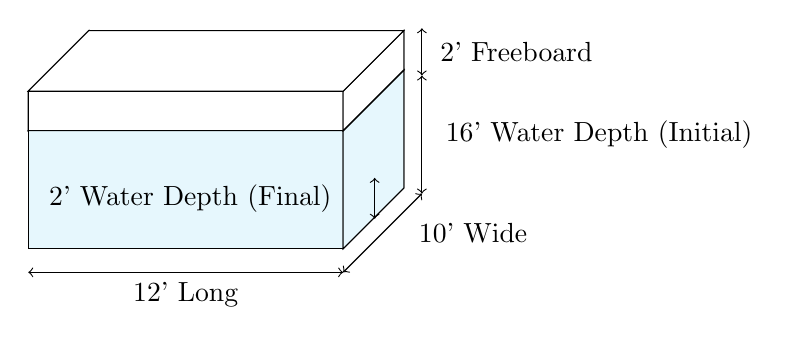
\begin{tikzpicture}

\pgfmathsetmacro{\cubexx}{4}
\pgfmathsetmacro{\cubeyy}{1.5}
\pgfmathsetmacro{\cubezz}{2}
\pgfmathsetmacro{\cubex}{4}
\pgfmathsetmacro{\cubey}{0.5}
\pgfmathsetmacro{\cubez}{2}
\pgfmathsetmacro{\cubexxx}{4}
\pgfmathsetmacro{\cubeyyy}{4}
\filldraw [fill=cyan!10!white, draw=black] (0,-\cubey,0) -- ++(-\cubexx,0,0) -- ++(0,-\cubeyy,0) -- ++(\cubexx,0,0) -- cycle ;
\filldraw [fill=cyan!0!white, draw=black] (0,-\cubey,0) -- ++(0,0,-\cubezz) -- ++(0,-\cubeyy,0) -- ++(0,0,\cubezz) -- cycle;
\filldraw [fill=cyan!10!white, draw=black] (0,-\cubey,0) -- ++(0,0,-\cubezz) -- ++(0,-\cubeyy,0) -- ++(0,0,\cubezz) -- cycle;
%\filldraw [fill=cyan!10!white, draw=black] (0,-\cubey,0) -- ++(-\cubexx,0,0) -- ++(0,0,-\cubezz) -- ++(\cubexx,0,0) -- cycle;
%%%\draw (0,-0.5,0) -- ++(-\cubex,0,0) -- ++(0,-\cubey,-\cubez) -- ++(\cubex,0,0) -- cycle;
\draw (-\cubex,0,0) -- ++(0,0,-\cubez) -- ++(0,-\cubey,0) -- ++(0,0,\cubez) -- cycle;
\draw (0,-\cubey,0) -- ++(-\cubex,0,0) -- ++(0,0,-\cubez) -- ++(\cubex,0,0) -- cycle;
\filldraw [fill=white, draw=black] (0,0,0) -- ++(-\cubex,0,0) -- ++(0,-\cubey,0) -- ++(\cubex,0,0) -- cycle ;
\filldraw [fill=white, draw=black] (0,0,0) -- ++(0,0,-\cubez) -- ++(0,-\cubey,0) -- ++(0,0,\cubez) -- cycle;
\filldraw [fill=white, draw=black] (0,0,0) -- ++(0,0,-\cubez) -- ++(0,-\cubey,0) -- ++(0,0,\cubez) -- cycle;
\filldraw [fill=white, draw=black] (0,0,0) -- ++(-\cubex,0,0) -- ++(0,0,-\cubez) -- ++(\cubex,0,0) -- cycle;

%\filldraw [fill=RoyalBlue!10!white, draw=black] (0,-1.5,0) -- ++(-\cubex,0,0) -- ++(0,-\cubey,0) -- ++(\cubex,0,0) -- cycle ;

%\filldraw [fill=RoyalBlue!10!white, draw=black] (0,-1.5,0) -- ++(0,0,-\cubez) -- ++(0,-\cubey,0) -- ++(0,0,\cubez) -- cycle;



%%\draw (0,-0.5,0) -- ++(-\cubex,0,0) -- ++(0,0,-\cubez) -- ++(\cubex,0,0) -- cycle;
%%\filldraw [fill=white, draw=black] (-\cubex,0,0) -- ++(0,0,-\cubez) -- ++(0,-\cubey,0) -- ++(0,0,\cubez) -- cycle;
%%\filldraw [fill=white, draw=black] (0,-\cubey,0) -- ++(-\cubex,0,0) -- ++(0,0,-\cubez) -- ++(\cubex,0,0) -- cycle ;

\draw [<->] (-4,-2.3) -- (0,-2.3) node [midway, below] {12' Long};
\draw [<->] (1,-1.3) -- (1,.2) node [midway, midway] {\hspace{4.5cm}16' Water Depth (Initial)};
\draw [<->] (0.4,-1.62) -- (0.4,-1.1) node [midway, midway] {\hspace{-4.8cm} 2' Water Depth (Final)};
\draw [<->] (1,.8) -- (1,.2) node [midway, midway] {\hspace{2.4cm}2' Freeboard};
\draw [<->] (1,-1.3) -- (0,-2.3) node [midway, midway] {\hspace{2.3cm}10' Wide};
\end{tikzpicture}\\
Volume to be pumped=$12 \enspace ft*10 \enspace ft *(16-2)\enspace ft=1,680ft^3$\\
\vspace{0.3cm}
$\implies \dfrac{1,680\cancel{ft^3}*7.48\dfrac{\cancel{gal}}{\cancel{ft^3}}}{600\dfrac{\cancel{gal}}{min}}=\boxed{21min}$

\item 1 MGD is pumped against a 14’ head.  What is the water Hp?  The pump mechanical efficiency is 85\%.  What is the brake horsepower?\\
\vspace{0.4cm}
water Hp = flow * head\\
\vspace{0.4cm}
$\dfrac{1,000,000 \enspace gal}{day}*\dfrac{day}{1440 \enspace min}*14 \enspace ft*\dfrac{Hp}{3,960 \enspace GPM-ft}=\boxed{Water \enspace Hp = 2.46 \enspace Hp}$\\
\vspace{0.4cm}
pump Hp = brake Hp * pump efficiency\\
\vspace{0.4cm}
$Brake \enspace Hp = \dfrac{2.46}{0.85}=\boxed{Brake \enspace Hp=2.89Hp}$\\

\vspace{0.4cm}

\item A 8 ft diameter cylindrical wetwell receives an average incoming flow if 135 gpm and is pumped down with a pump that delivers 450 gpm again a total dynamic head of 120 ft.  The pump is controlled using two floats; a stop float located at 2.5 ft and a start float located at 16 ft.  If the pump motor is rated at 88\% and the pump at 77\%, what is the monthly (30 days/month) for running this pump if power costs are \$0.11/Kwh?\\


\vspace{0.4cm}
When the pump is on, the volume of wetwell that will be pumped down with the 450 gpm pump and a 135 gpm flow to the wetwell:\\
\vspace{0.4cm}
$\dfrac{450 \enspace gal}{min}-\dfrac{135 \enspace gal}{min}=\dfrac{315 \enspace gal}{min}$\\
\vspace{0.4cm}
Minutes required to pump down the wetwell :\\
\vspace{0.4cm}
$0.785*8^2*(16-2.5)ft^3*\dfrac{7.48 \enspace gal}{ft^3}*\dfrac{min}{315 \enspace gal}=16.1 \enspace min$\\
\vspace{0.4cm}
Time to fill wetwell with pump off @135gal/min influent flow:
\\
\vspace{0.4cm}
$[0.785*8^2*(16-2.5)]ft^3*\dfrac{7.48 \enspace gal}{ft^3}*\dfrac{min}{135 \enspace gal}=37.6min$\\
\vspace{0.4cm}
\# of cycles per day:\\
\vspace{0.4cm}
$\dfrac{cycle}{(16.1+37.6) \enspace min}*\dfrac{1440 \enspace min}{day}=\dfrac{26.8 \enspace cycles}{day}$\\
\vspace{0.4cm}
\# of hrs pump operational:\\
\vspace{0.4cm}
$\dfrac{16.1 \enspace min}{cycle}*\dfrac{26.8 \enspace cycles}{day}*\dfrac{hrs}{60 \enspace min}=\dfrac{7.19 \enspace hours}{day}$\\
\vspace{0.4cm}
Monthly electrical cost:\\
\vspace{0.4cm}
$\dfrac{450 \enspace gpm*120 \enspace ft}{0.88*0.77}*\dfrac{Hp}{3,960 \enspace gpm-ft}*\dfrac{0.746 \enspace kW}{Hp}*\dfrac{7.19hrs}{day}*\dfrac{30 \enspace days}{month}*\dfrac{\$0.11}{kWh}=\boxed{\dfrac{\$356}{month}}$\\
\vspace{0.4cm}

\item A 6-year old pump motor is to be replaced at a net cost of \$15,800. The new motor, just like the old one, would run 65\% of the time. Both existing and replacement motors would operate at 125 output Hp. The existing motor efficiency is 86\% while the replacement motor would be guaranteed at 94\% efficiency. Electricity currently averages \$0.088 per kWh.\\
\vspace{0.4cm}
(a) Calculate the energy cost savings per year (to the nearest dollar) if the existing motor is replaced with the new motor (neglect any consideration of impact upon demand charges or interest on capital).\\
\vspace{0.4cm}
(b) What is payback period to the nearest tenth of a year.\\
\vspace{0.4cm}
Solution:\\
\vspace{0.4cm}
Calculate energy cost savings per year:\\
\vspace{0.4cm}
Input Hp for old motor:$\dfrac{125}{0.86}=145.35Hp$\\
\vspace{0.4cm}
Input Hp for old motor:$\dfrac{125}{0.94}=132.98Hp$\\
\vspace{0.4cm}
Energy cost savings:\\$(145.35-132.98)Hp*\dfrac{0.746 \enspace kW}{Hp}*\dfrac{(365*24*0.65)hrs}{yr}*\dfrac{\$0.088}{kWh}=\boxed{\dfrac{\$4,624}{yr}}$\\
\vspace{0.4cm}
Calculate payback:\\
\vspace{0.4cm}
$\$15,800*\dfrac{yr}{\$4,623.94}=\boxed{3.4yr}$


\item A flow of 200 gpm  is pumped against a total head of 4.0 feet. The pump is 78\% efficient and the motor' is 90\% efficient. Calculate the input Hp.\\
\vspace{0.4cm}
water Hp = flow * head\\
\vspace{0.2cm}
$200GPM*4ft*\dfrac{Hp}{3,960 GPM-ft}=0.2Hp$\\
\vspace{0.4cm}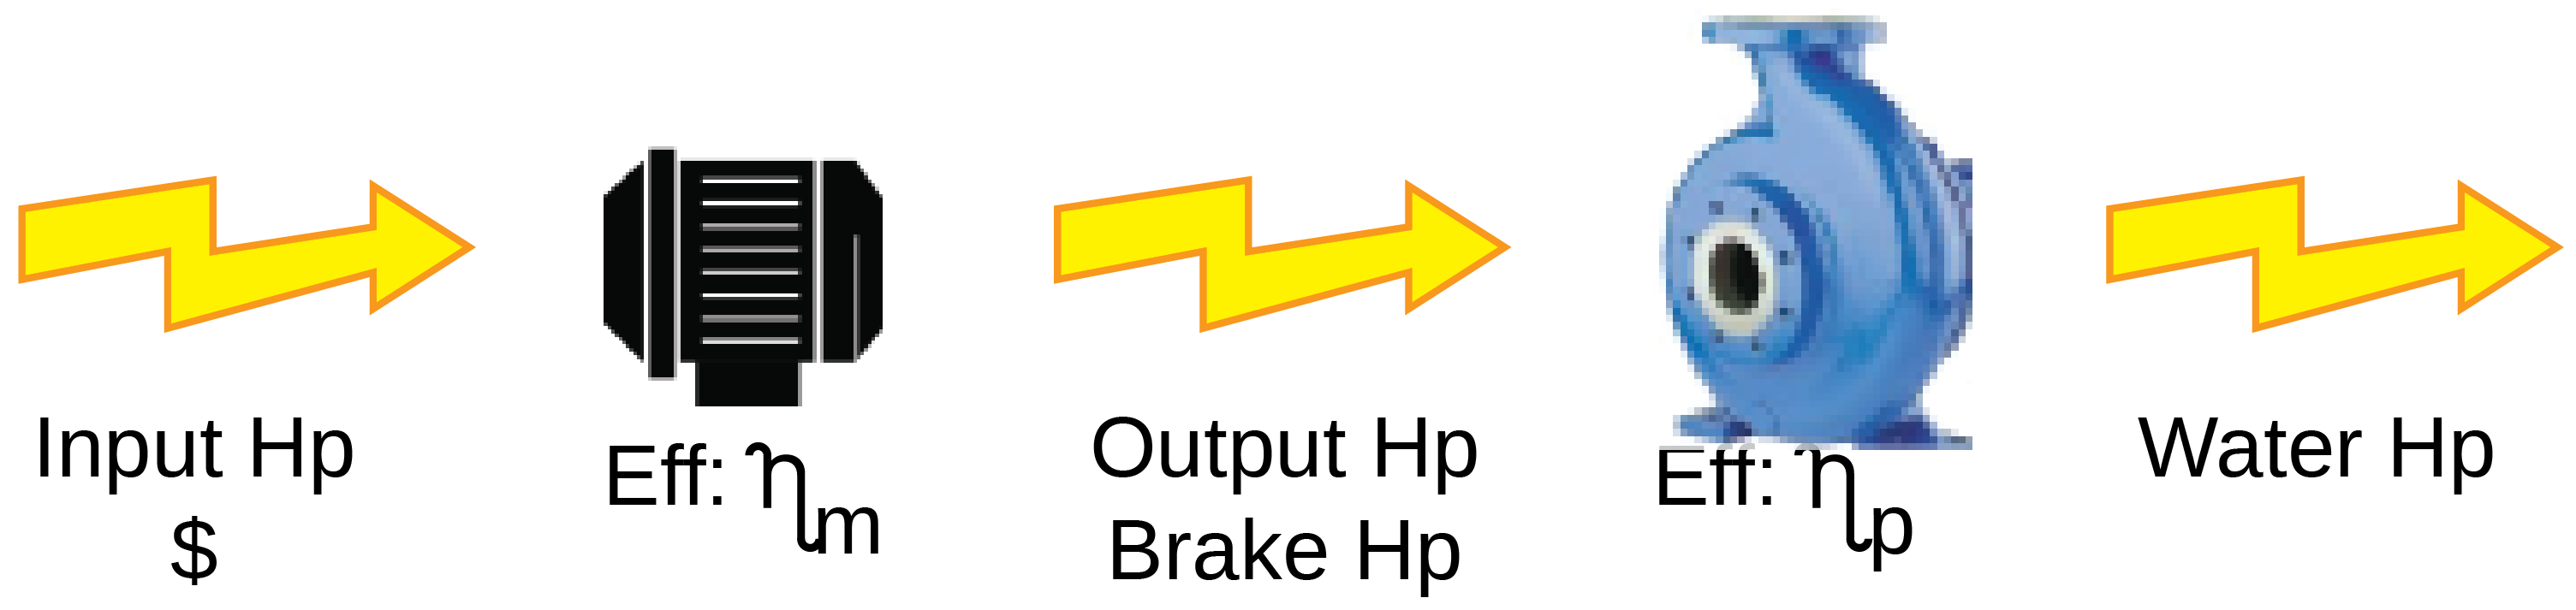
\includegraphics[scale=0.08]{PumpProblem}\\
water Hp=brake Hp*pump efficiency, and\\
brake Hp=input Hp*motor efficiency\\
Therefore, water Hp=input Hp*motor efficiency*pump efficiency\\
\vspace{0.4cm}
input Hp=$\dfrac{water \enspace Hp}{motor \enspace efficiency*pump \enspace efficiency}=\dfrac{0.2}{0.9*0.78}=\boxed{0.28Hp}$
\vspace{0.2cm}
\end{enumerate}






\newpage
\section*{Chapter Assessment}
\begin{tcolorbox}[breakable, enhanced,
colframe=blue!25,
colback=blue!10,
coltitle=blue!20!black,  
title= Chapter Assessment]

\begin{enumerate}
\item The chemical used for each day during a week is given below. Based on these data, what was the average lb/day chemical used during the week?\\

\begin{tabular}{|l|l|}
\hline
Monday & 92 lb/day\\
\hline
Tuesday & 93 lb/day \\
\hline
Wednesday & 98 lb/day\\
\hline
Thursday & 93 lb/day \\
\hline
Friday & 89 lb/day\\
\hline
Saturday & 93 lb/day \\
\hline
Sunday & 97 lb/day\\
\hline
\end{tabular}

\item The average day winter demand of a community is 14,500 gallons. If the summer demand is estimated to be $72 \%$ greater than the winter, what is the estimated summer demand? 


\item A 60-foot diameter tank contains 422,000 gallons of water. Calculate the height of water in the storage tank.

\item How much paint will it take for a single coat of the top and sidewalls of the storage tank that is 100-feet in diameter and 30-feet tall, if one gallon of paint covers 200 square feet?\\

\item A tank has a diameter of 60 feet with an overflow depth at 44 feet. The current water level is 16 feet. Water is flowing into the tank at a rate of 250 gallons per minute. At this rate, how many days will it take to fill the tank to the overflow?

\item A rectangular channel 3 ft. wide contains water 2 ft. deep flowing at a velocity of 1.5 fps.
What is the flow rate in cfs?

\item On an average, 2 inches of grit is collected and removed every day in a 2.2 feet wide, 205 feet long grit channel.  Knowing the average flow through that grit channel is 10 MGD calculate the rate of grit collection in ft$^3$/MG\\


\item A clarifier has a TSS removal efficiency of 50\%.  If the influent TSS concentration is 220 mg/L, how many lbs/day of TSS are removed if the flow is 10 MGD.  Also, how many cu. ft of sludge is pumped if the sludge has a TS concentration of 5\%.\\


\item What is the surface loading rate (gal/(day-sq.ft) of a 15 MGD flow in a 105 ft diameter primary sedimentation tank operating at water depth of 20 ft.\\

\item  A 12 MGD primary clarifier effluent flow is fed to a trickling filter. If the total flow to the trickling filter including the recirculated flow is 17 MGD, what is the recirculation ratio? \\

\item The flow to a pond is 7.2MGD. If the pond diameter is 350 ft and the BOD in the pond influent is 170mg/L, what is the organic loading to this pond in lbs BOD/day/acre?

\item How deep must a 60 acre facultative pond be operated in order to have a detention time of 45 days. Flow to the pond is 2.0 MGD. 

\item In an aeration tank, the MLSS is 2500 mg/l and recorded 30-minute settling test for a 1-litre MLSS samples indicates 230 ml of settled solids. What is the sludge volume index?

\item The desired F/M ratio is .35lbs BOD/day/lb MLVSS.  If 2,100 lbs of BOD enter the aerator daily, how many lbs of MLVSS should be maintained in the aeration tank? \\ 

\item Given the following data, calculate the mean cell residence time (MCRT)\\
DATA: \\
Influent flow= 35 MGD\\
MLSS = 2850 mg/L\\
Waste sludge flow = 0.08 MGD\\
Total secondary system volume= 20 MG\\
Waste activated sludge suspended solids conc. = 6000 mg/L\\
Final effluent suspended solids = 25 mg/L \\

\item 42,000 gallons of 6\% sludge containing 67\% volatile matter is pumped to the digester.  The digester reduces the volatile matter by 52\%.  What volume of sludge in gallons containing 5\% solids remains after digestion? 

\item How much gas is produced in the above digester in $ft^3$/day if the digested sludge contains 2.5\% total solids of which 59\% is volatile solids and the gas production rate is 14 $ft^3$/lb VS destroyed?\\

\item A belt press is used for dewatering 70 GPM digested sludge containing 3\% TS, seven hours per day.  At the end of the day it produces 24 $yd^3$ of 16\% TS \enspace biosolids @ 65 lbs/$ft^3$ density.  What is the percent belt press solids recovery?\\

\item Calculate the air required (SCFM) to meet a 0.04 lb air:lb feed solids ratio for a 100 GPM WAS flow with a solids content of 6500mg/l? Assume 0.08 lbs air/SCF air.\\

\item Calculate how many pounds per day of chlorine should be used to maintain a dosage of 12 mg/l at a 5.0 MGD flow.\\

\item The operator at a 1.5 MGD conventional activated sludge plant is considering using either HTH or sodium hypochlorite as an alternative to chlorine gas. Currently chlorine is being dosed at 15 mg/L in order to achieve a residual of 3.0 mg/L. Using the data provided below calculate the daily cost for chlorine, HTH, and sodium hypochlorite (NaOCl) (Sp.Gravity 1.21).
 
Chlorine $\rightarrow$ 0.15 \$/lb\\
HTH (70\% available chlorine) $\rightarrow$ 0.25 \$/lb\\
NaOCl (15\% available chlorine) $\rightarrow$ 0.35 \$/gal 


\item Liquid alum (49\% alum, sp. gravity 1.32, \$1.85/gal)) is being used to remove phosphorus from a 600,000 gpd activated sludge effluent. Two hundred milligrams per liter (200 mg/L) of alum, $Al_2(S0_4)_3.14H_20$, is required to give adequate removal of the phosphorus in this effluent. Calculate the daily cost of liquid alum needed to remove phosphorus. [Formula Weights: Al =27, $Al_2(S0_4)_3.14H_20$ =594]\\

\item Find the brake horsepower for a pump given the following information: Total Dynamic Head $=75$ feet, Pump Rate $=150$ gpm, Pump Efficiency $=90 \%$, Motor Efficiency $=85 \%$

\end{enumerate}
\end{tcolorbox}
















